\documentclass[11pt,a4paper]{article}
\usepackage[utf8]{inputenc}
\usepackage[T1]{fontenc}
\usepackage[brazilian]{babel}
\usepackage{geometry}
\geometry{margin=2.5cm}
\usepackage{graphicx}
\usepackage{booktabs}
\usepackage{float}
\usepackage{hyperref}
\usepackage{xcolor}
\usepackage{amsmath}

\title{Documentação Operacional da Pipeline de Detecção de Anomalias\\
\large Turbina A -- Cabiúnas}
\author{Equipe de Modelagem}
\date{Setembro de 2026}

\begin{document}
\maketitle

\begin{abstract}
Este documento descreve, de forma operacional e reproduzível, a
pipeline final de detecção de anomalias adotada como configuração de
produção: como os três modelos especializados são montados e
configurados, como o treinamento é conduzido, o que acontece depois
do treinamento (portões de produção, canalização binária, votação,
filtro de duração mínima, refratário) e o resultado final sobre o
histórico de TRIPs disponível. Todas as figuras e tabelas foram
geradas a partir do retreino completo dos três modelos (03/09/2026) e
do estudo dos falsos positivos residuais (04/09/2026), que resultou
na adição do filtro de duração mínima de 45 minutos na votação
combinada.
\end{abstract}

\tableofcontents

\section{Visão geral}

A pipeline combina \textbf{3 modelos especializados} (um por
mecanismo físico: temperatura de mancal, vibração de mancal, pressão
de óleo) com \textbf{1 canal estatístico sem modelo} (proximidade
temporal a alarmes de processo já catalogados), cujas saídas binárias
são combinadas por uma camada de decisão de regras fixas (votação e
refratário). A Figura~\ref{fig:arquitetura} mostra a arquitetura
completa, ponta a ponta.

\begin{figure}[H]
\centering
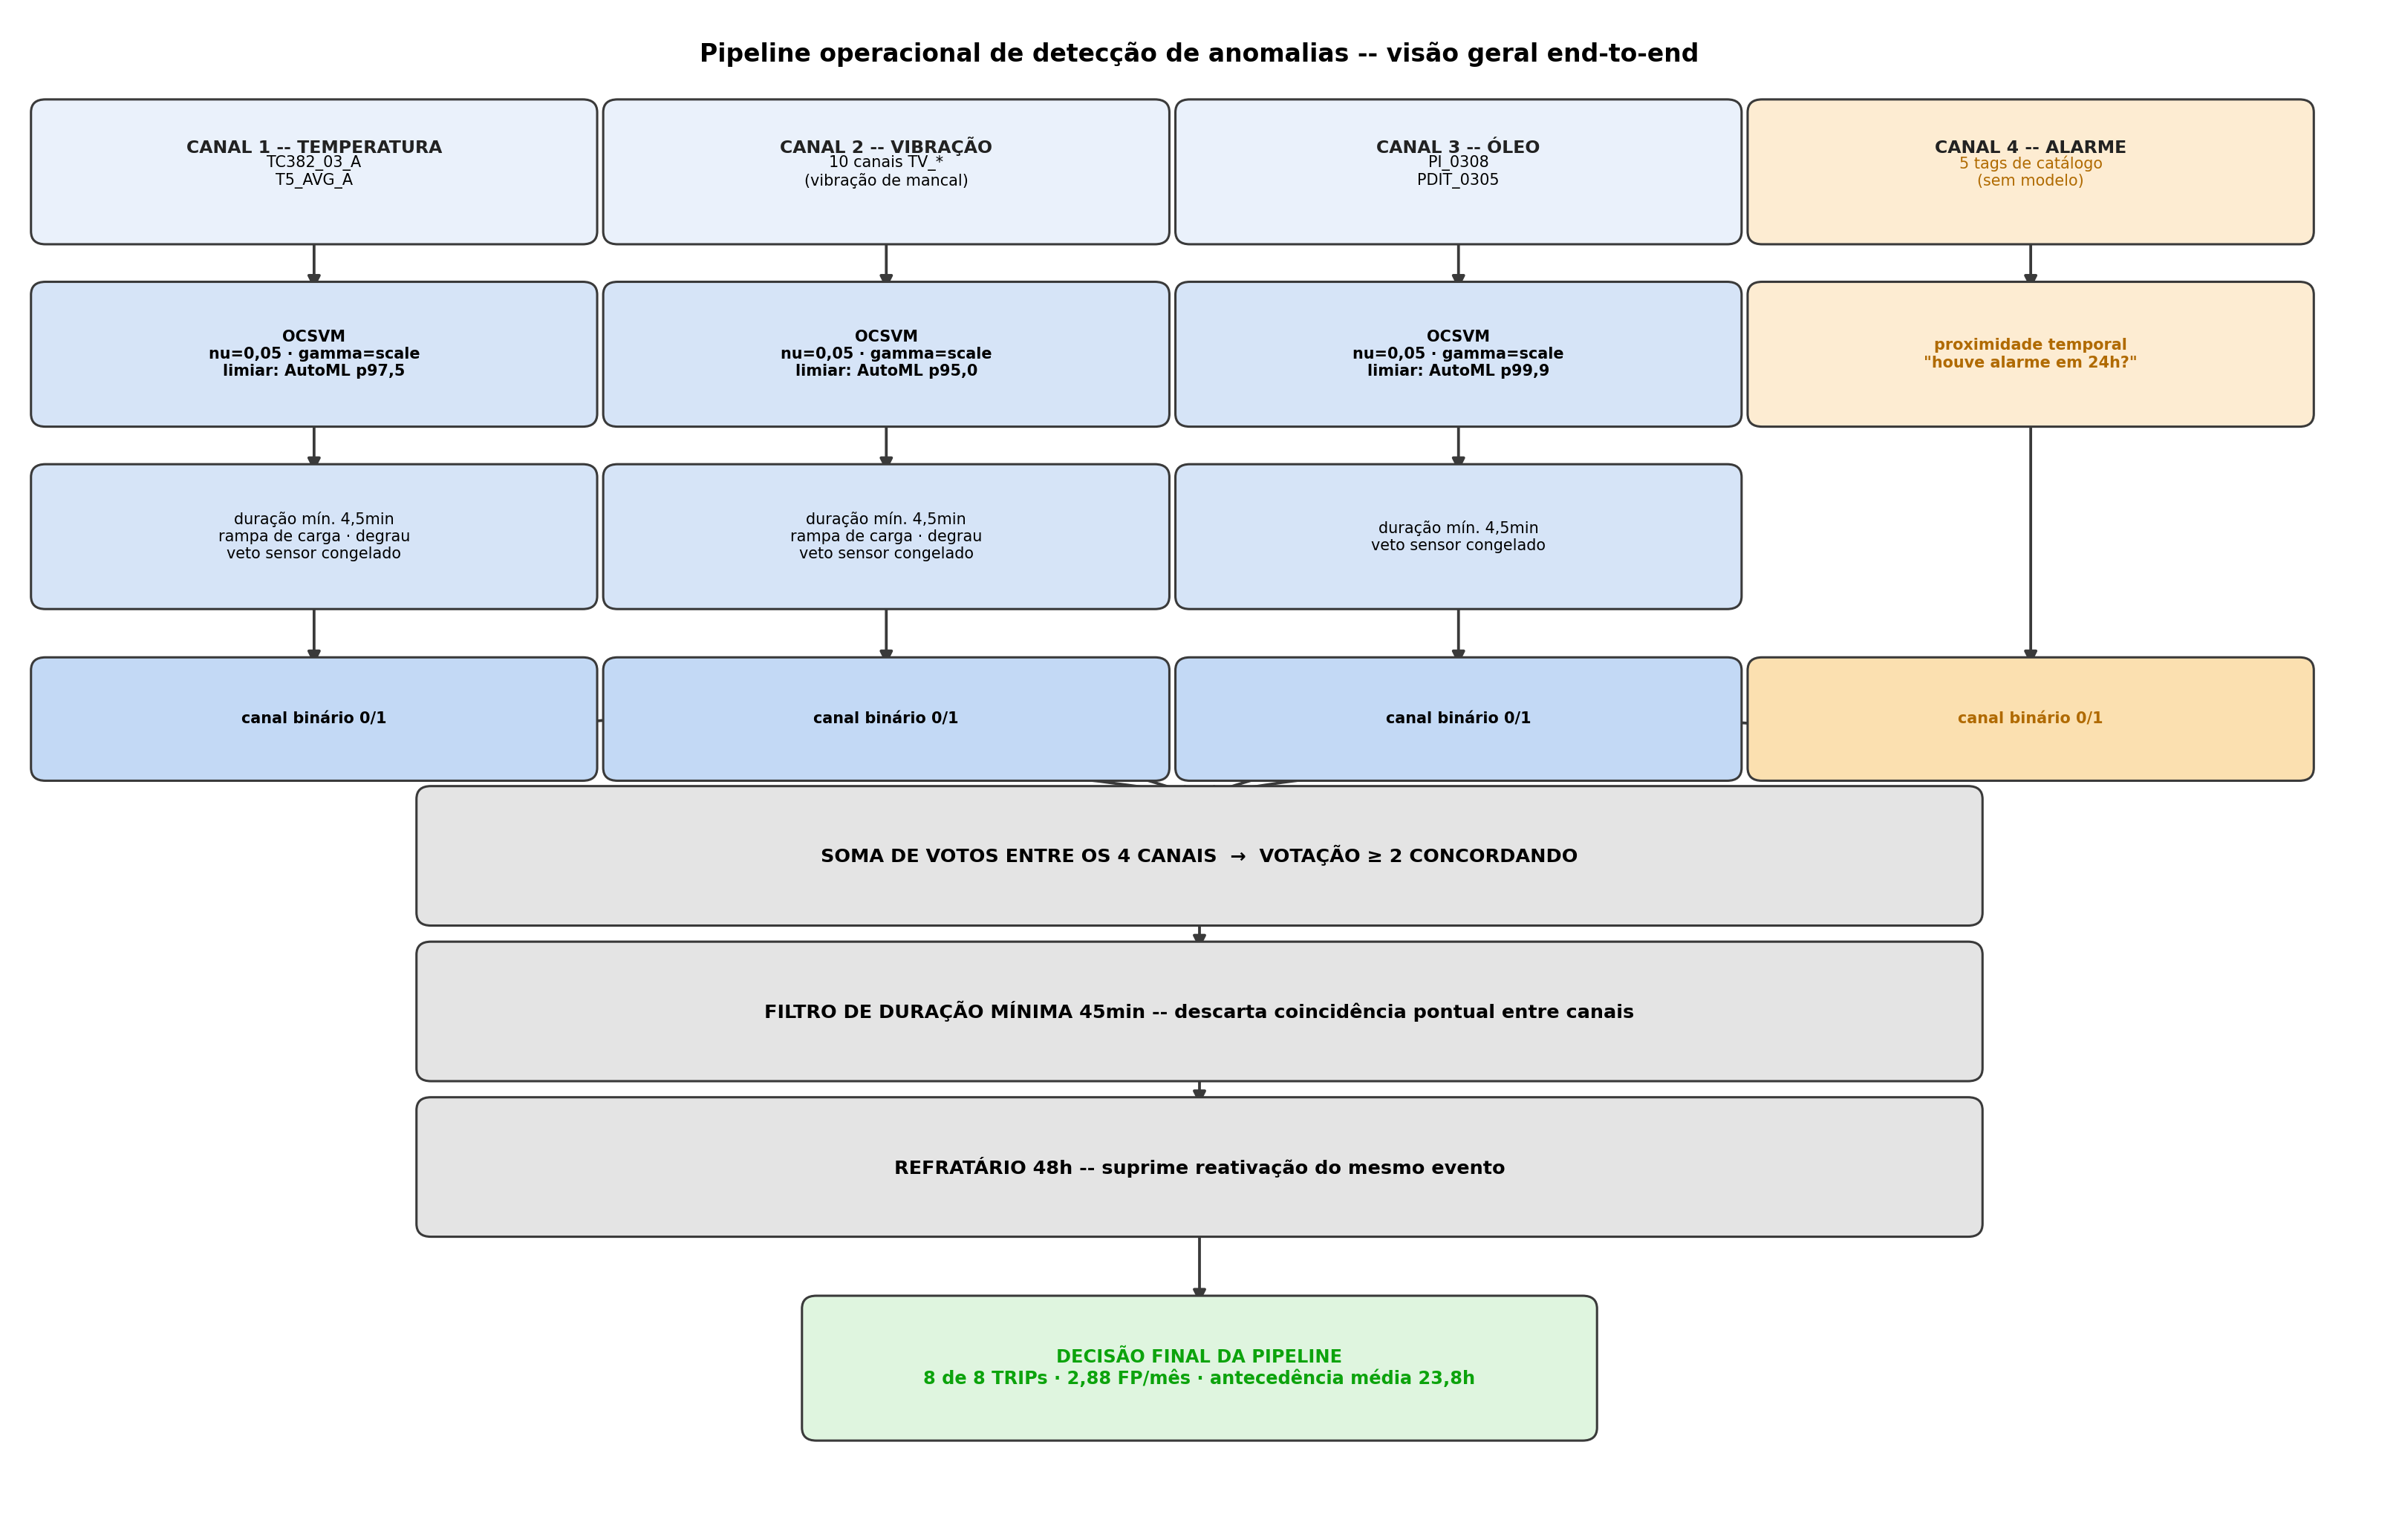
\includegraphics[width=\textwidth]{diagrama_pipeline_operacional.png}
\caption{Arquitetura end-to-end da pipeline operacional: 4 canais
(3 modelos + 1 estatístico), portões de produção, votação e
refratário.}
\label{fig:arquitetura}
\end{figure}

\section{Como a pipeline é montada}

\subsection{Separação de sinais por canal}

Cada canal modelado vê apenas os sensores do seu próprio mecanismo
físico -- essa separação (em vez de um único modelo recebendo todos
os sinais juntos) é o que permite que cada modelo seja sensível ao
seu próprio regime de anomalia, sem diluição por variação normal de
outros mecanismos.

\begin{table}[H]
\centering
\begin{tabular}{lll}
\toprule
\textbf{Canal} & \textbf{Sensores usados} & \textbf{Sensor alvo} \\
\midrule
1 -- Temperatura & TC382\_03\_A, T5\_AVG\_A & TC382\_03\_A \\
2 -- Vibração & 10 canais TV\_351X/Y\_A ... TV\_355X/Y\_A & TV\_351X\_A \\
3 -- Óleo & PI\_0308, PDIT\_0305 & PI\_0308 \\
4 -- Alarme de processo & 5 tags de catálogo (sem sensor contínuo) & -- \\
\bottomrule
\end{tabular}
\caption{Separação de sensores por canal. Nenhum canal modelado
compartilha sensores com outro.}
\end{table}

\subsection{Configuração de treinamento}

Os três canais modelados usam o mesmo algoritmo (\textit{One-Class
SVM}), a mesma janela de dados e o mesmo procedimento de calibração
por AutoML (busca de limiar de anomalia e debounce por grade,
validação fora da amostra). O que muda entre eles é apenas o escopo
de sensores e, em alguns casos, quais portões de produção fazem
sentido fisicamente para aquele mecanismo.

\begin{table}[H]
\centering
\small
\begin{tabular}{lccc}
\toprule
\textbf{Parâmetro} & \textbf{Temperatura} & \textbf{Vibração} & \textbf{Óleo} \\
\midrule
Modelo & OCSVM & OCSVM & OCSVM \\
$\nu$ (nu) & 0,05 & 0,05 & 0,05 \\
$\gamma$ (gamma) & scale & scale & scale \\
Máx. amostras de treino & 50.000 & 50.000 & 50.000 \\
Grade de percentil (limiar) & 95 -- 99,9 & 69 -- 99,9 & 69 -- 99,9 \\
Grade de debounce (min) & 1, 4, 12 & 1, 4, 12 & 1, 4, 12 \\
Janela de dados & \multicolumn{3}{c}{01/07/2024 -- 20/04/2026} \\
Split fora-da-amostra & \multicolumn{3}{c}{a partir de 01/07/2025} \\
\midrule
Filtro de duração mínima & 4,5 min & 4,5 min & 4,5 min \\
Veto de sensor congelado & 30 min & 30 min & 30 min \\
Portão de degrau (T5\_AVG\_A) & sim & sim & não \\
Portão de rampa de carga (T5\_AVG\_A) & sim & sim & não \\
Portão de volatilidade & não & não & não \\
\bottomrule
\end{tabular}
\caption{Configuração de treinamento por canal. A grade de percentil
de temperatura é mais restrita porque o sinal já vive em percentis
altos; vibração e óleo usam uma grade ampliada (desde p69) para não
descartar precursores fracos que vivem em percentis mais baixos.}
\end{table}

O canal de alarme de processo não tem parâmetro treinado: é uma
verificação direta de proximidade temporal (``houve um alarme de uma
das 5 tags catalogadas nas últimas 24h?''), contra o catálogo
\texttt{alarmes\_selecionados\_turbina\_a.csv}, tags
\texttt{PI\_6240319\_AL}, \texttt{PAL\_6240315},
\texttt{PDAL\_6240302}, \texttt{TC382\_05\_A}, \texttt{PAH\_6240319}.

\subsection{Resultado do treinamento (calibração por AutoML)}

Para cada canal, a etapa de AutoML varre a grade de percentil de
limiar e debounce, escolhe a combinação com melhor pontuação composta
(taxa de detecção contra alarmes de referência, penalizada por falso
alarme) e valida fora da amostra.

\begin{table}[H]
\centering
\small
\begin{tabular}{lccc}
\toprule
\textbf{Métrica de calibração} & \textbf{Temperatura} & \textbf{Vibração} & \textbf{Óleo} \\
\midrule
Limiar escolhido (percentil) & p97,5 & p95,0 & p99,9 \\
Valor do limiar (erro OCSVM) & 10,50 & 0,176 & 29,67 \\
Debounce escolhido & 1 min & 4 min & 12 min \\
Nº de combinações testadas & 15 & 27 & 27 \\
Taxa de detecção (val. interna) & 92,5\% & 87,5\% & 100\% \\
Taxa de alarme em período normal & 0,68\% & 10,06\% & 0,27\% \\
Pontos normais usados no ajuste & 386.492 & 386.492 & 574.951 \\
\bottomrule
\end{tabular}
\caption{Resultado da calibração AutoML por canal, retreino de
03/09/2026. Essas métricas são internas ao próprio canal (contra seus
alarmes de referência), antes da votação final -- não confundir com
o resultado da régua rigorosa apresentado na Seção~\ref{sec:resultado}.}
\end{table}

\begin{figure}[H]
\centering
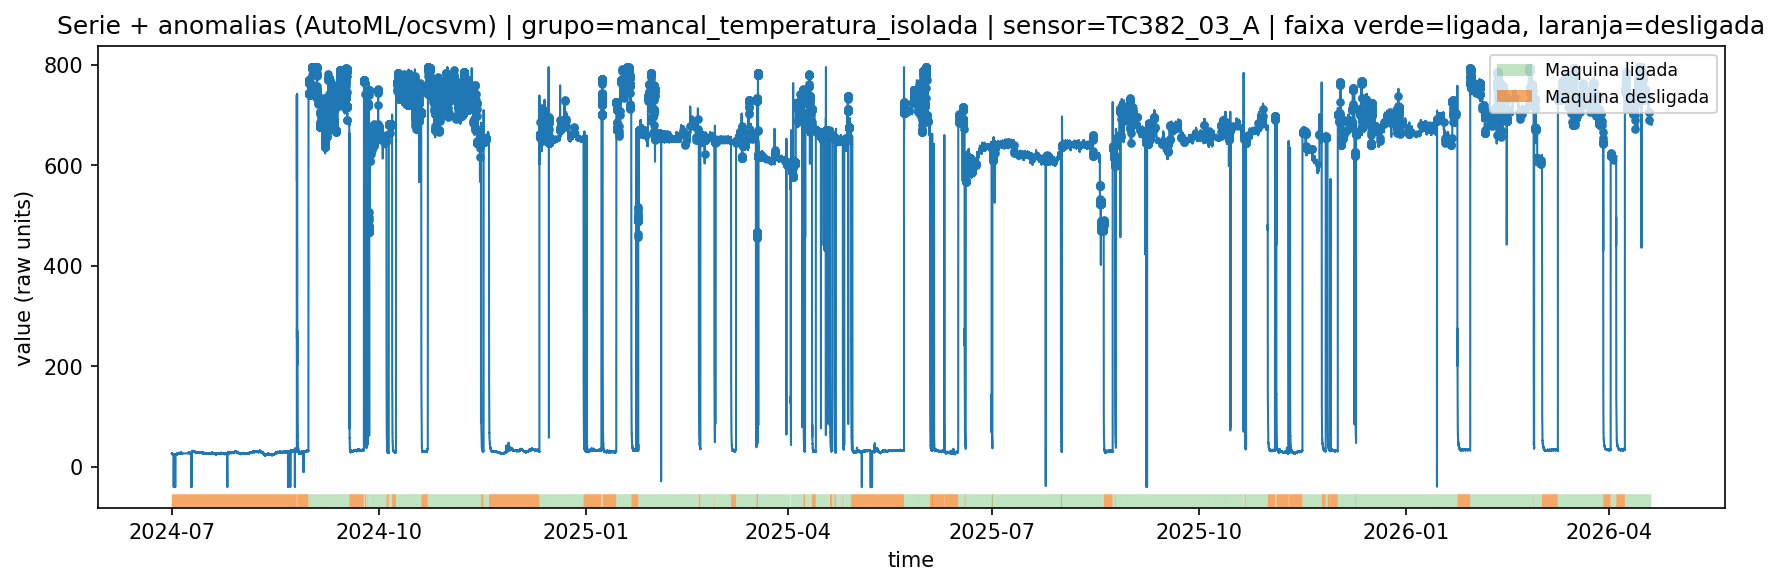
\includegraphics[width=0.85\textwidth]{treino_temperatura.png}
\caption{Canal 1 (temperatura) -- série com anomalias marcadas ao
final do treinamento e calibração.}
\end{figure}

\begin{figure}[H]
\centering
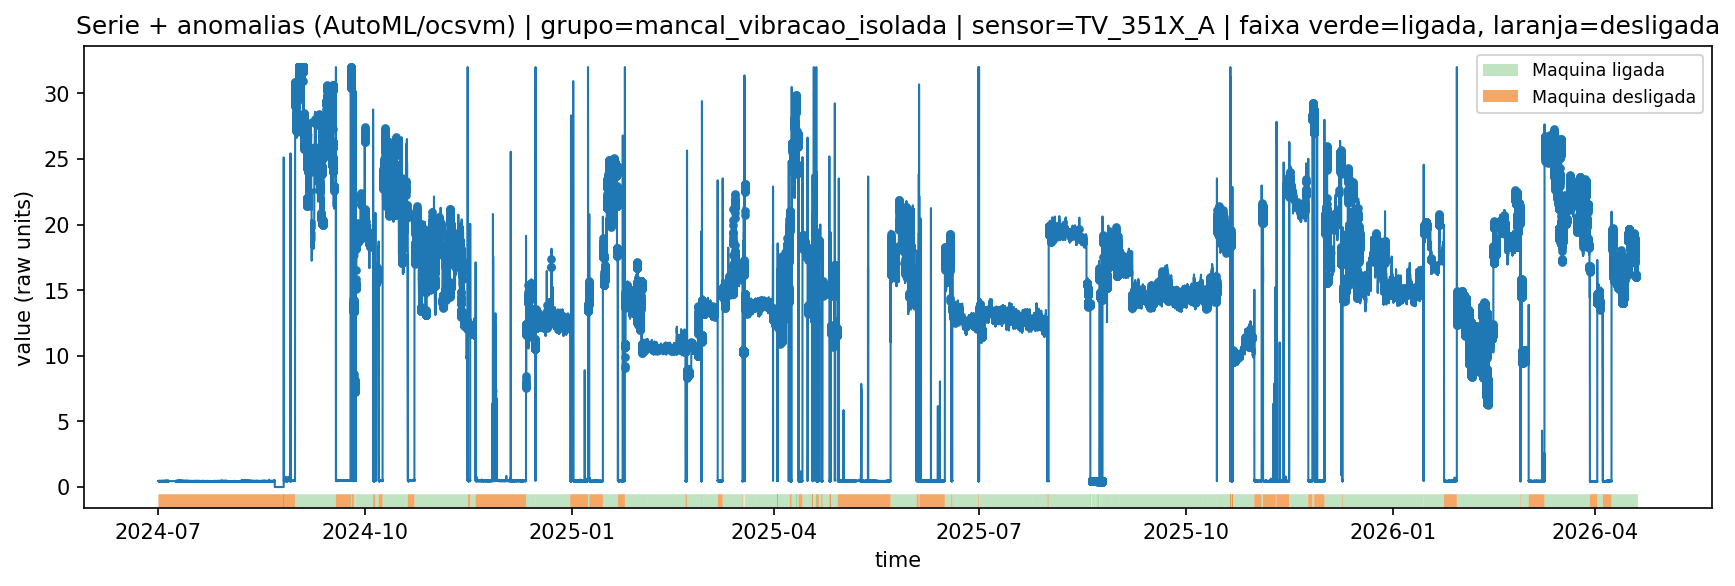
\includegraphics[width=0.85\textwidth]{treino_vibracao.png}
\caption{Canal 2 (vibração) -- série com anomalias marcadas ao final
do treinamento e calibração.}
\end{figure}

\begin{figure}[H]
\centering
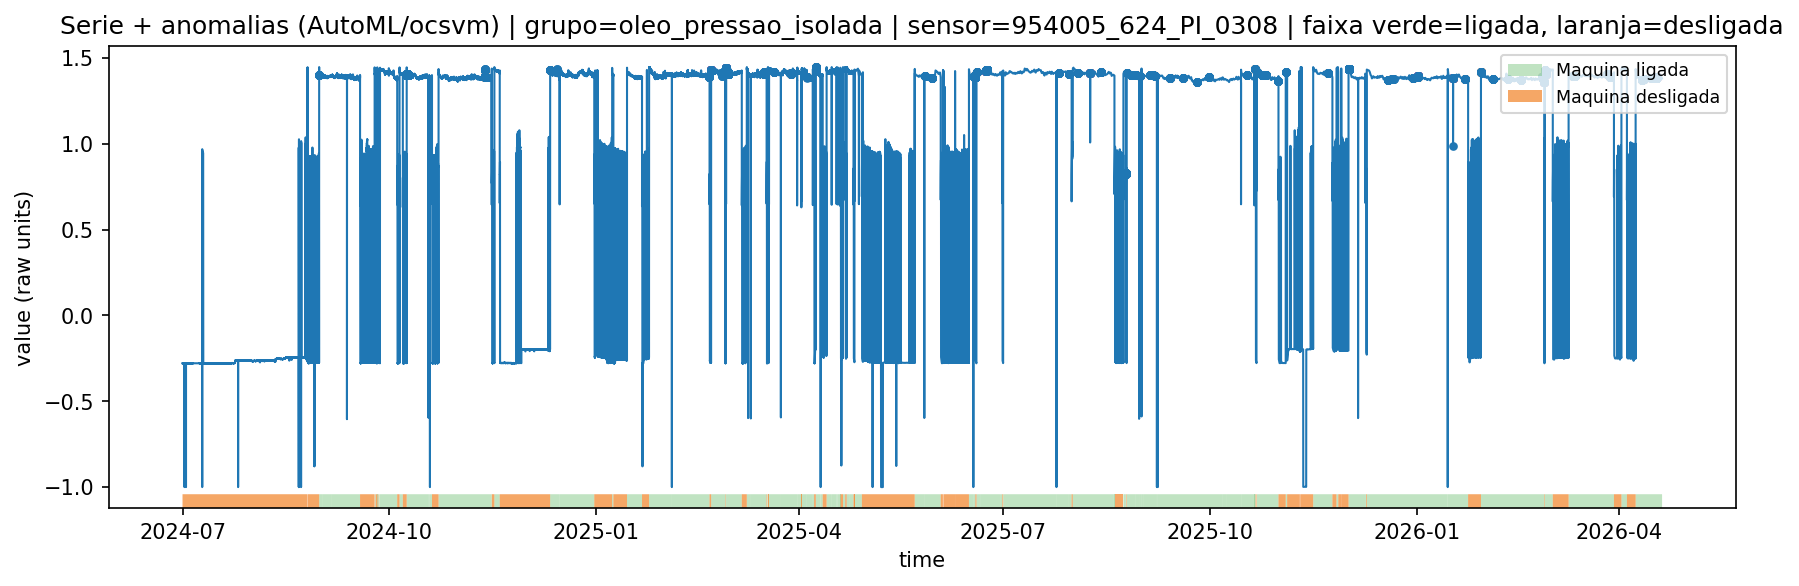
\includegraphics[width=0.85\textwidth]{treino_oleo.png}
\caption{Canal 3 (óleo) -- série com anomalias marcadas ao final do
treinamento e calibração.}
\end{figure}

\section{O que é feito depois do treinamento}

O modelo treinado de cada canal produz um \textbf{score contínuo} de
anomalia (erro de reconstrução/distância à fronteira do OCSVM).
Esse score passa por uma sequência de etapas antes de virar o
``voto'' binário do canal:

\begin{enumerate}
  \item \textbf{Limiar calibrado}: o score é comparado ao limiar
    escolhido pelo AutoML (Tabela acima) -- acima do limiar por pelo
    menos o tempo de debounce, o ponto é candidato a anomalia.
  \item \textbf{Portões de produção}: cada candidato passa por filtro
    de duração mínima (4,5 min), veto de sensor congelado, e, quando
    aplicável ao mecanismo (temperatura e vibração), portão de
    degrau e de rampa de carga -- isso suprime falsos alarmes
    causados por transientes operacionais normais (partida, parada,
    mudança de carga), não por anomalia real.
  \item \textbf{Canal binário}: o que sobra depois dos portões é o
    canal binário (0/1) daquele mecanismo -- é isso que entra na
    votação.
  \item \textbf{Votação}: os 4 canais binários (3 modelados + 1
    estatístico) são somados ponto a ponto; a decisão bruta é
    ``ativa'' quando \textbf{pelo menos 2 dos 4} concordam no mesmo
    instante.
  \item \textbf{Filtro de duração mínima (45 min)}: aplicado sobre a
    votação combinada -- descarta episódios de concordância
    \emph{pontual} entre canais (coincidências de segundos a poucos
    minutos) que não representam um evento físico sustentado. Ver
    justificativa e varredura de segurança na
    Seção~\ref{sec:estudo-fp}.
  \item \textbf{Refratário}: uma vez que a decisão dispara, novas
    ativações do mesmo evento são suprimidas por 48h -- isso evita
    que um único evento físico prolongado gere múltiplos alarmes
    repetidos.
\end{enumerate}

A Figura~\ref{fig:passoapasso} ilustra essa sequência sobre uma
janela real (o TRIP de 04/11/2025): no Passo 1 cada canal acende de
forma independente e em instantes diferentes; no Passo 2 a soma de
votos cruza o limiar de 2 pouco antes do TRIP; no Passo 3 o filtro de
duração mínima mantém apenas o trecho sustentado da votação; no Passo
4 a decisão final dispara uma única vez (verde) e fica suprimida pelo
refratário até o TRIP acontecer (linha roxa).

\begin{figure}[H]
\centering
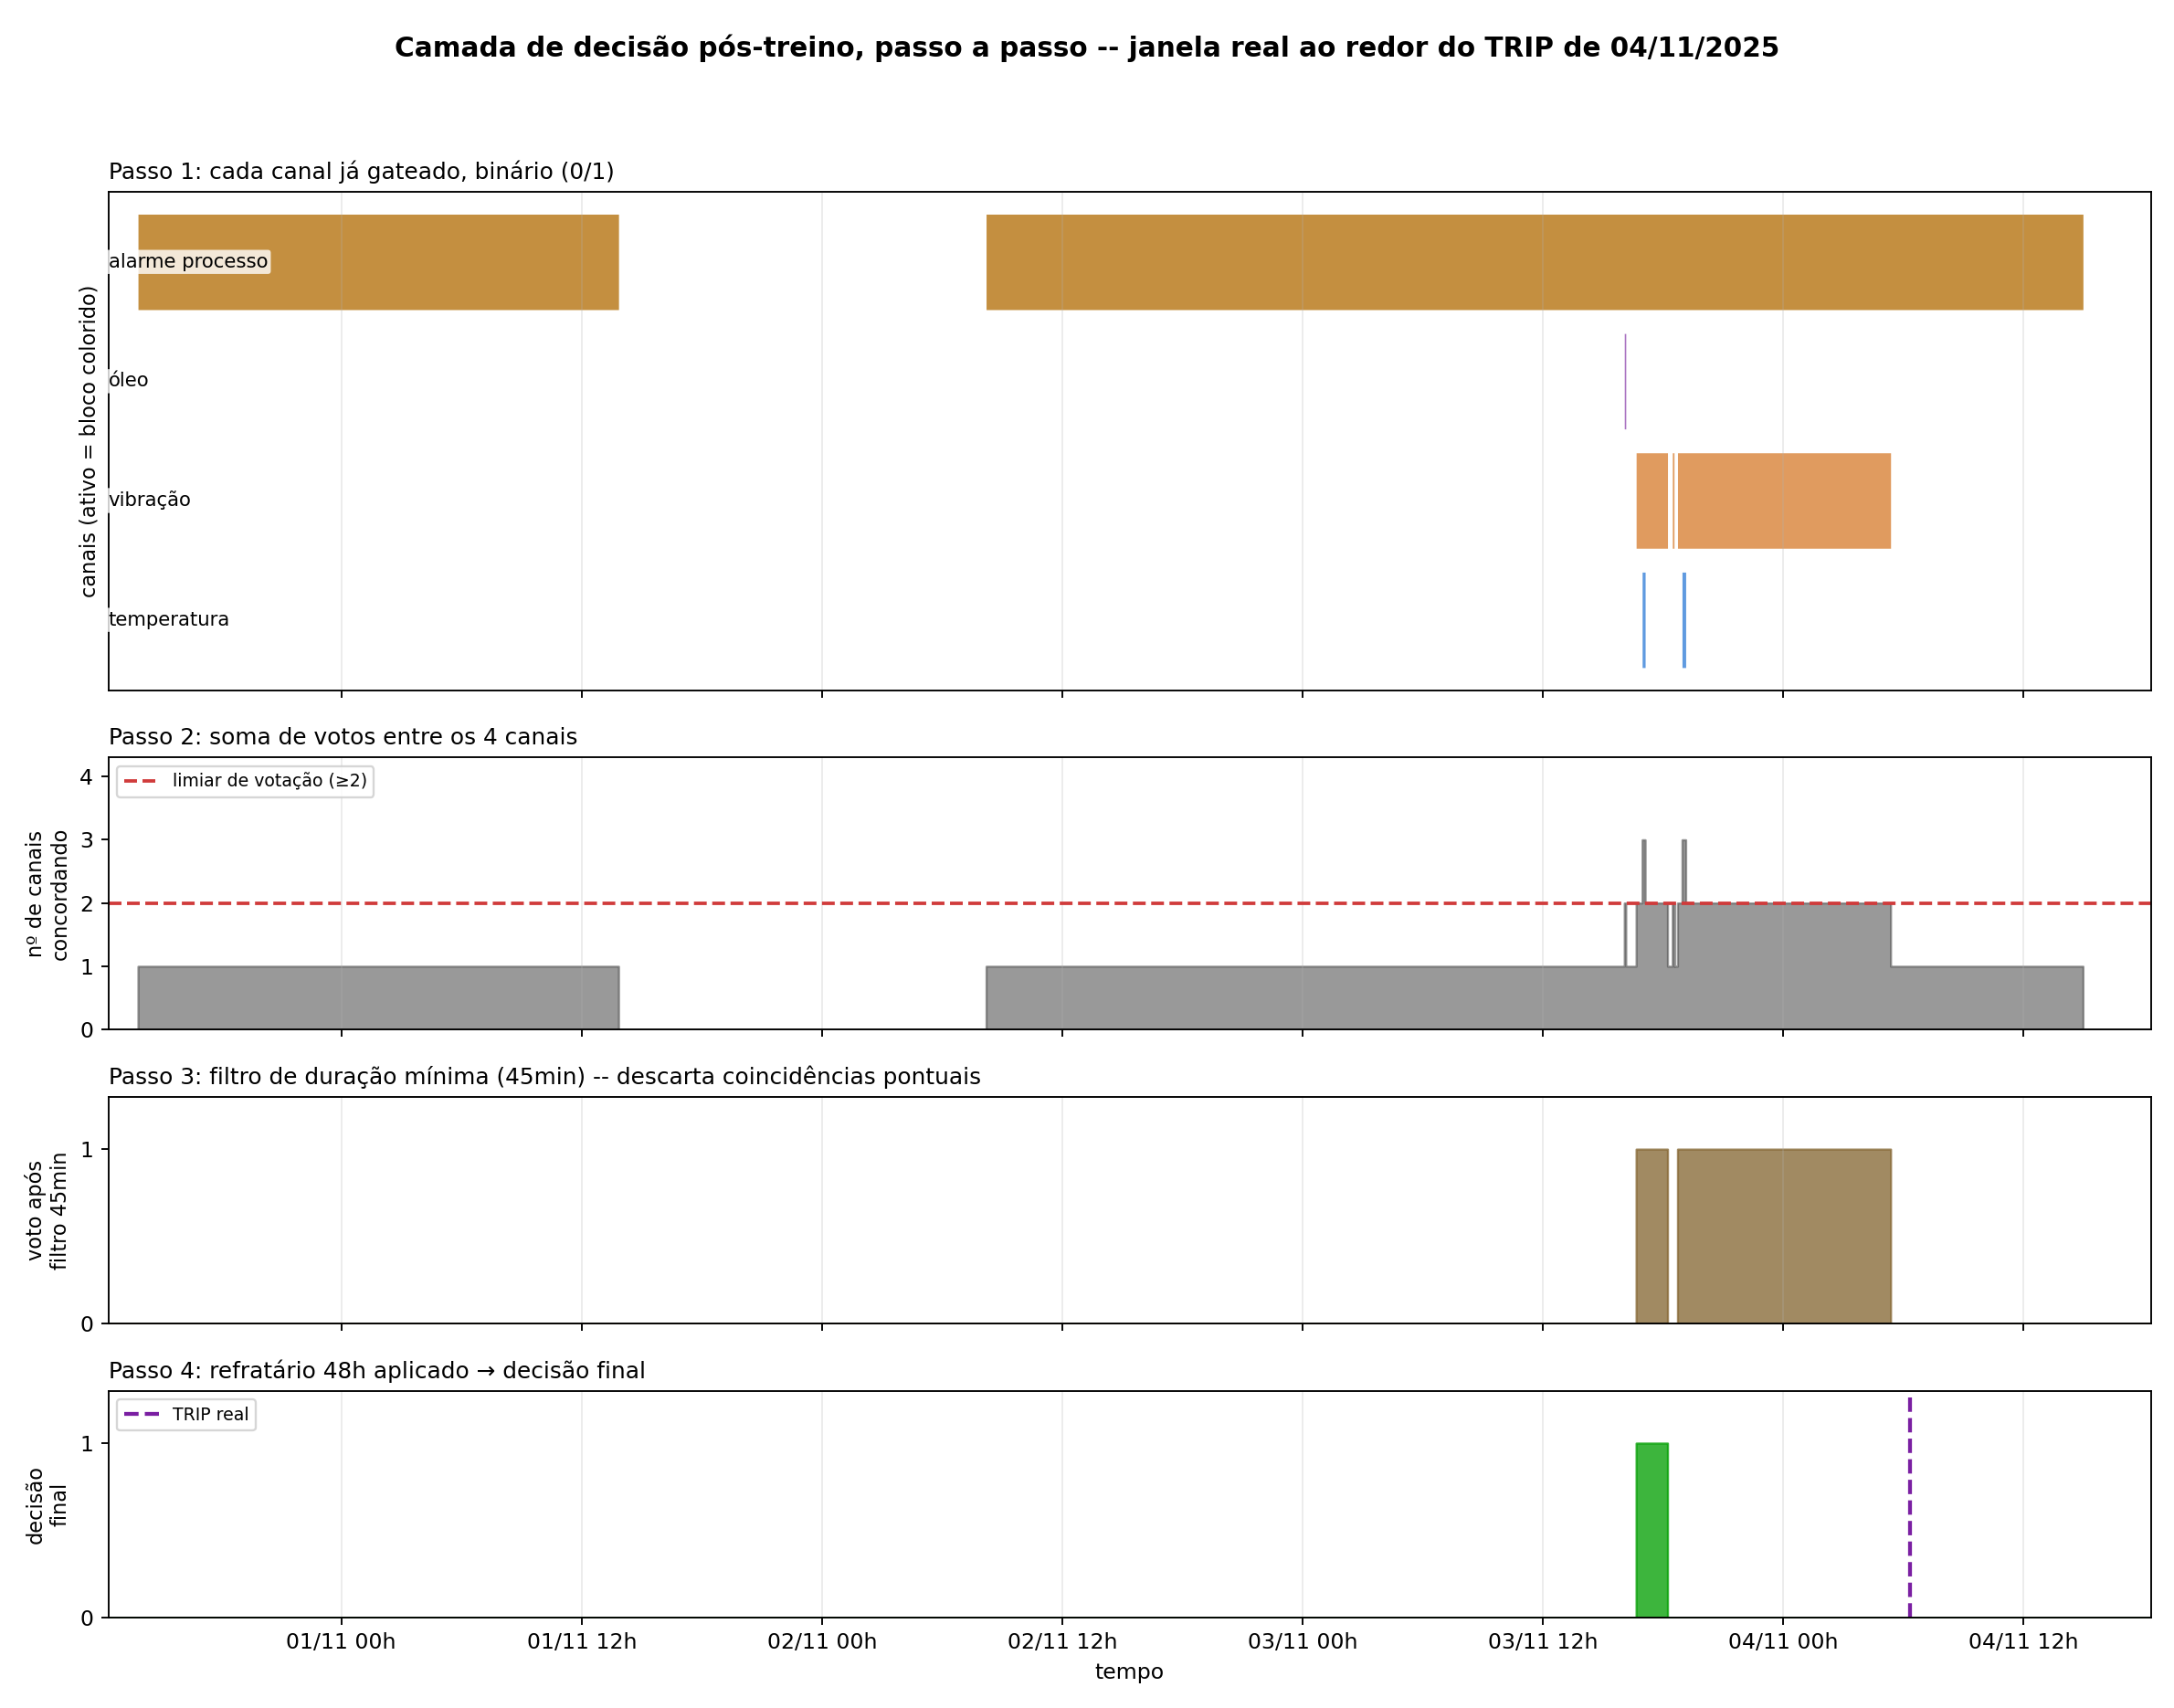
\includegraphics[width=\textwidth]{passo_a_passo_decisao.png}
\caption{Passo a passo da camada de decisão pós-treino, sobre uma
janela real de TRIP.}
\label{fig:passoapasso}
\end{figure}

\section{Estudo dos falsos positivos e filtro de duração mínima}
\label{sec:estudo-fp}

Antes de aceitar qualquer mudança para reduzir falso positivo, os 96
episódios de FP da configuração anterior (votação ≥2 + refratário,
sem filtro de duração) foram caracterizados pela combinação de canais
que os disparou:

\begin{table}[H]
\centering
\begin{tabular}{lcc}
\toprule
\textbf{Combinação de canais} & \textbf{Nº de episódios} & \textbf{Duração mediana} \\
\midrule
Temperatura + Alarme & 27 & $\sim$30s \\
Vibração + Alarme & 26 & $\sim$12min \\
Temperatura + Vibração & 22 & $\sim$45s \\
Temperatura + Vibração + Alarme & 12 & $\sim$1,4h \\
Óleo + Alarme & 6 & $\sim$45min \\
Temp.+Vib.+Óleo+Alarme & 2 & $\sim$1,9h \\
Vibração + Óleo + Alarme & 1 & 1,2h \\
\bottomrule
\end{tabular}
\caption{Caracterização dos 96 FP por combinação de canais (config.
sem filtro de duração). Mais da metade (49 de 96) tem duração
mediana abaixo de 1 minuto -- coincidência pontual entre canais já
individualmente filtrados, não sinal sustentado.}
\end{table}

Isso motivou testar um filtro de duração mínima na votação combinada
(análogo ao já usado em cada canal individualmente), varrendo o
limiar de duração contra a régua rigorosa \textbf{antes} de adotar
qualquer valor:

\begin{table}[H]
\centering
\small
\begin{tabular}{cccl}
\toprule
\textbf{Duração mín.} & \textbf{TRIPs} & \textbf{FP/mês} & \textbf{Observação} \\
\midrule
0 min (sem filtro) & 8/8 & 6,59 & configuração anterior \\
14--15 min & 7/8 & 4,3 & zona de fronteira instável (ver texto) \\
16 a 52 min & \textbf{8/8} & 4,19 a 2,68 & \textbf{platô seguro, verificado ponto a ponto} \\
55 min & 7/8 & 2,54 & quebra permanente começa aqui \\
58--60 min & 5/8 & 2,4--2,5 & 3 TRIPs perdidos \\
\midrule
\textbf{45 min (escolhido)} & \textbf{8/8} & \textbf{2,88} & margem de 10min do início da quebra \\
\bottomrule
\end{tabular}
\caption{Varredura de duração mínima na votação combinada, 04/09/2026.
A zona instável em 14--15min corresponde ao TRIP de 11/04/2025, que já
era conhecido como caso de fronteira (detectado com apenas 2 votos, a
0,9h de um religamento da máquina) -- volta a 8/8 logo acima, e o
valor final (45min) fica com folga de ambos os lados.}
\end{table}

\textbf{Decisão: filtro de duração mínima de 45 minutos}, aplicado à
votação combinada antes do refratário. Reduz FP/mês de 6,59 para
\textbf{2,88 (-56\%)} e episódios inconclusivos de 42 para 25, sem
perder nenhum dos 8 TRIPs -- com margem de segurança verificada, não
apenas extrapolada, dos dois lados do limiar escolhido.

Uma ideia alternativa avaliada e \textbf{rejeitada} nesta mesma
investigação foi suprimir alarmes nas primeiras 6h após a máquina
religar (prática usada por outros pesquisadores no mesmo contexto):
20 dos 96 FP caíam nessa janela, mas 2 dos 8 TRIPs reais também
disparavam dentro dela (a 0h e a 0,9h de um religamento) -- uma
supressão cega os teria eliminado junto. O filtro de duração mínima
resolve o mesmo tipo de ruído sem esse efeito colateral, porque ataca
a característica real do ruído (duração) em vez de uma
correlação temporal aproximada (proximidade a um religamento).

\subsection{Efeito visual do filtro: mecanismo e antes/depois na série completa}

A Figura~\ref{fig:mecanismo} mostra o mecanismo em um exemplo real e
isolado (14/08/2025): temperatura e vibração cruzam seus limiares ao
mesmo tempo por menos de 1 minuto -- sem o filtro, esse instante
seria um alarme (curva vermelha); com o filtro de 45min, a
coincidência nunca chega a se sustentar e o resultado fica em zero
(curva verde). Não há dados de outros canais nem eventos próximos
nesta janela -- é uma coincidência pontual isolada, exatamente o tipo
de ruído que o filtro foi desenhado para eliminar.

\begin{figure}[H]
\centering
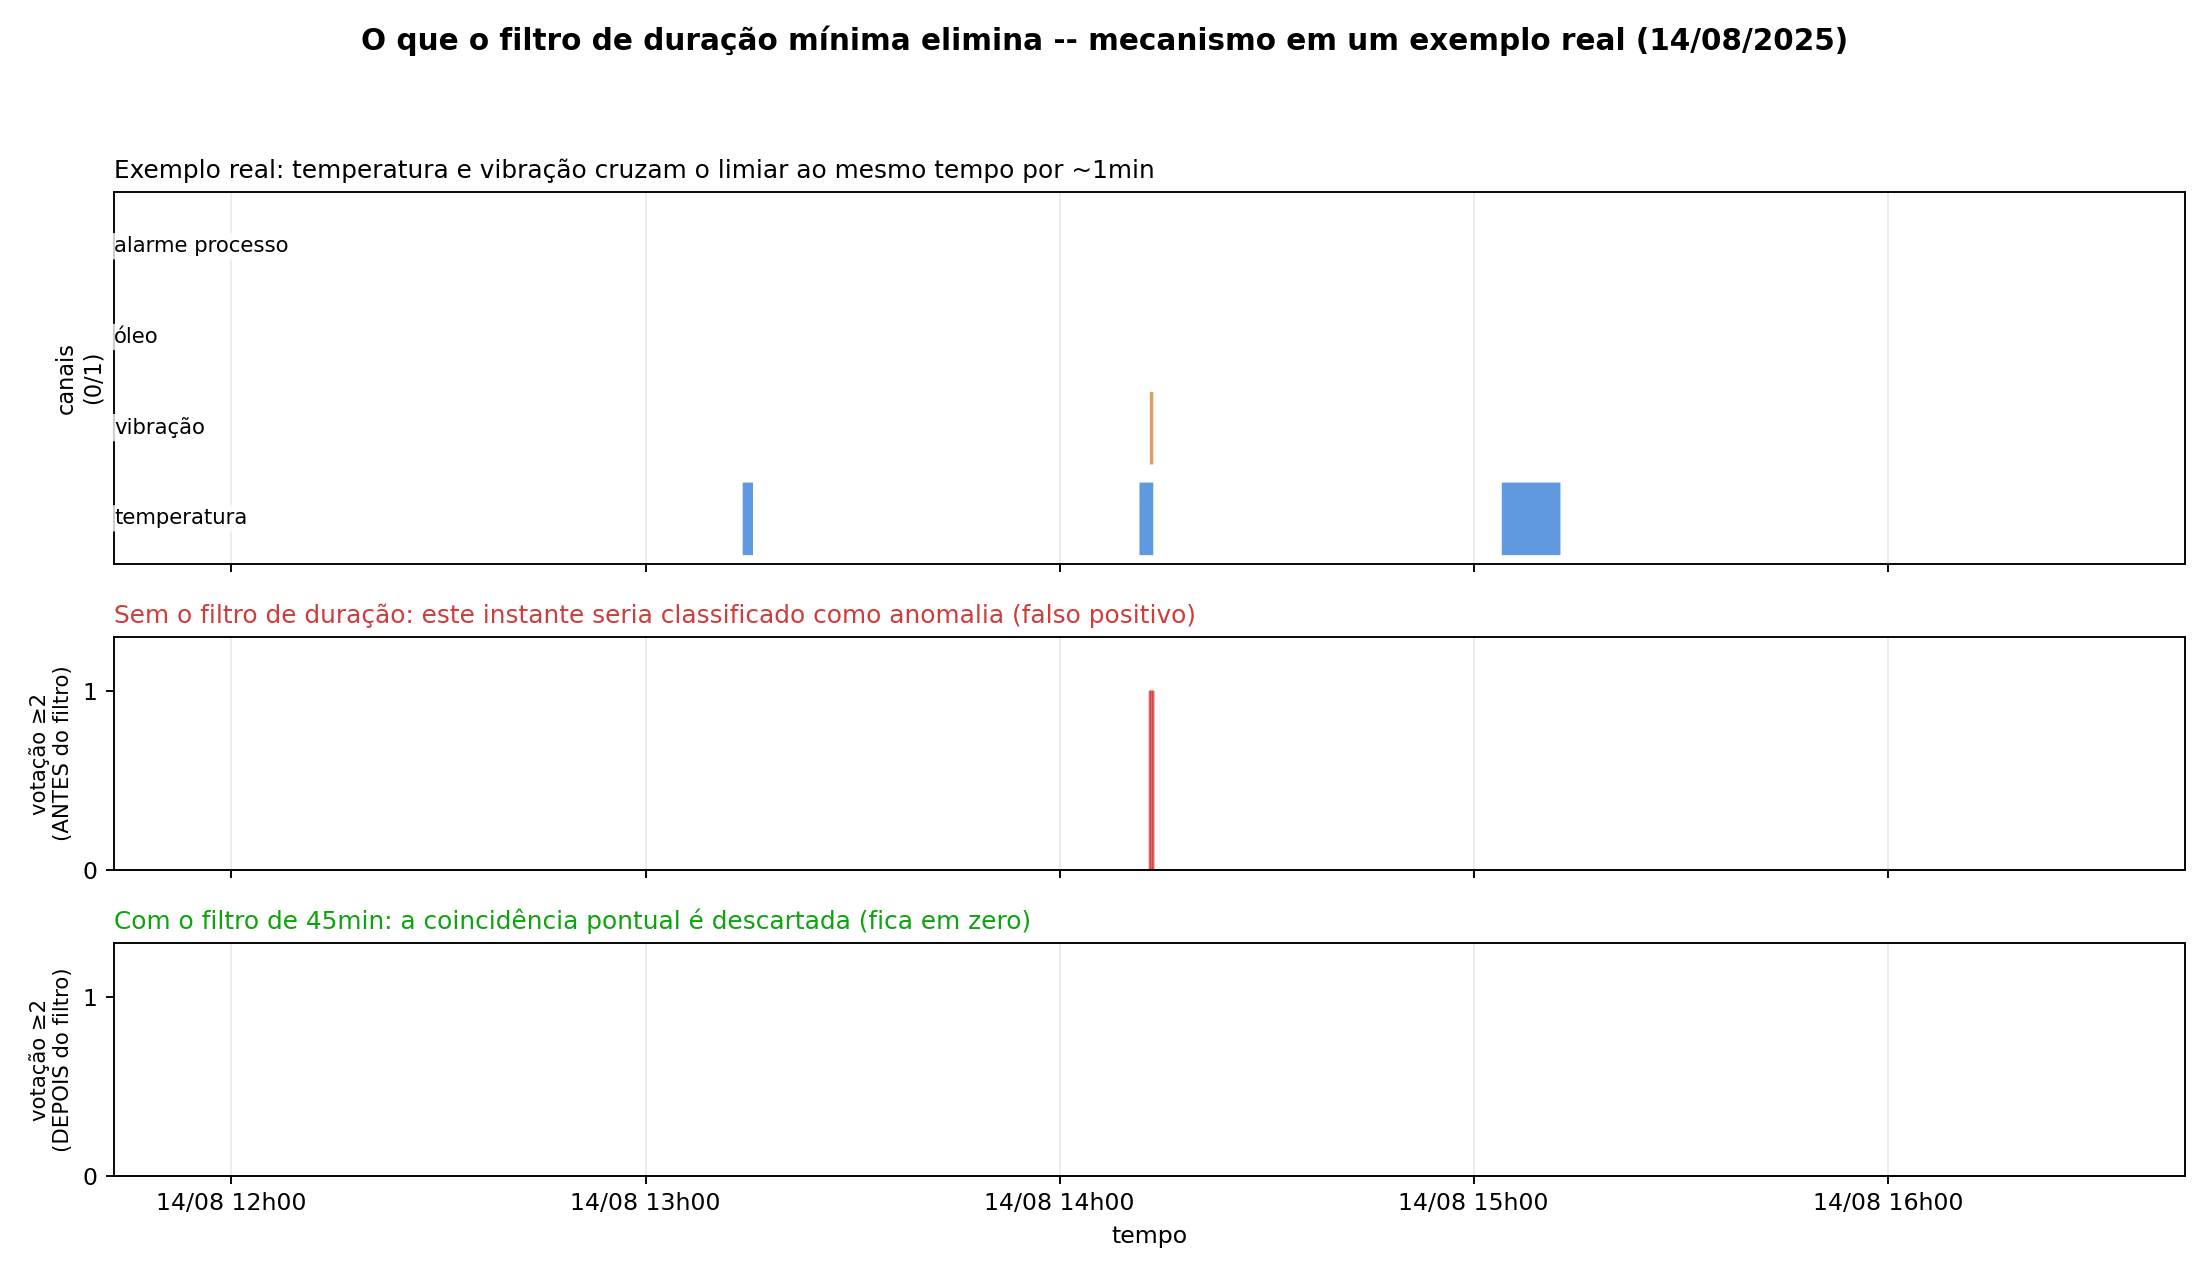
\includegraphics[width=\textwidth]{mecanismo_filtro_duracao.png}
\caption{Mecanismo do filtro de duração mínima em um exemplo real e
isolado: a votação bruta (vermelho) dispara por menos de 1 minuto; o
filtro de 45min descarta essa coincidência (verde, permanece em
zero).}
\label{fig:mecanismo}
\end{figure}

A Figura~\ref{fig:antesdepois} mostra o mesmo efeito sobre a série
inteira (não apenas um exemplo): em laranja, todos os pontos que
seriam classificados como anomalia \emph{antes} do filtro e que o
filtro de 45min elimina; em preto, os que sobrevivem (falso positivo
remanescente); em verde, os 8 acertos de TRIP; em roxo, as ocorrências
reais de TRIP. O volume de laranja domina visualmente sobre o preto
em quase todos os episódios -- é a mesma redução de 56\% (6,59 para
2,88 FP/mês) vista ponto a ponto ao longo dos $\sim$22 meses de dados.

\begin{figure}[H]
\centering
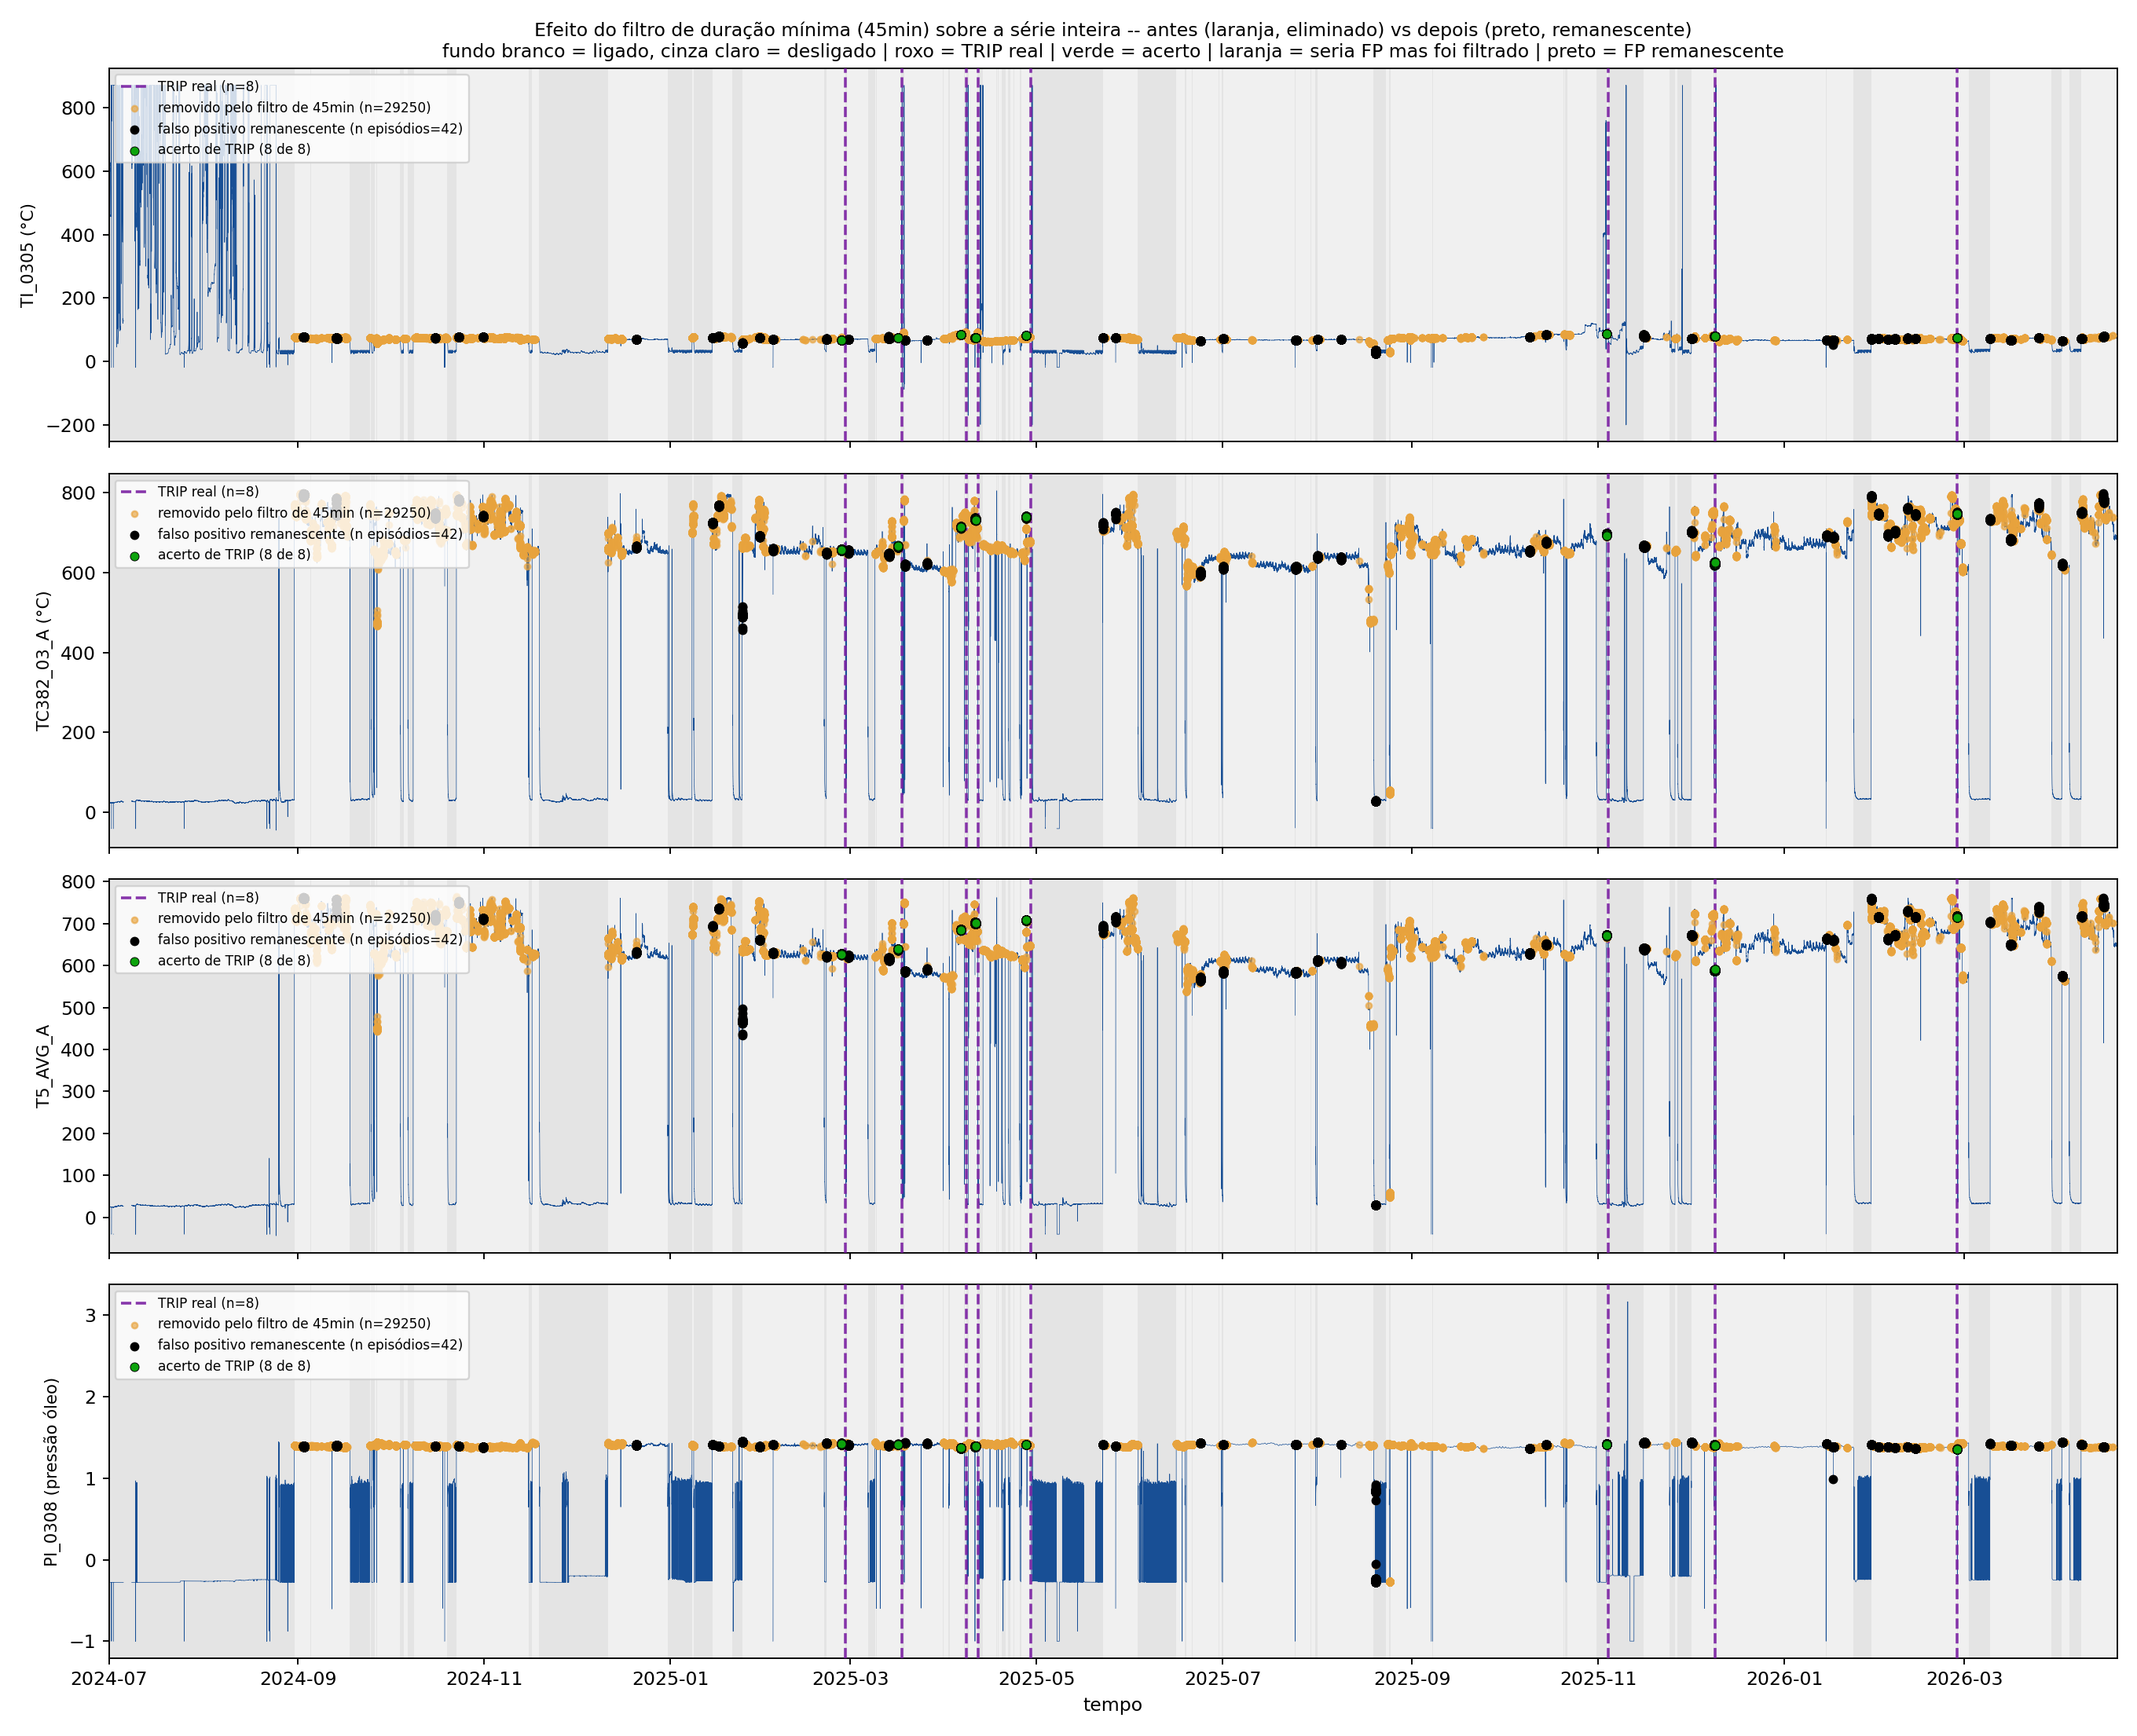
\includegraphics[width=\textwidth]{serie_antes_depois_filtro.png}
\caption{Série bruta completa (TI\_0305, TC382\_03\_A, T5\_AVG\_A,
PI\_0308) com os pontos que o filtro de 45min elimina (laranja, n=29.250
pontos) sobrepostos aos que permanecem como falso positivo (preto) e
aos 8 acertos de TRIP (verde). As linhas verticais roxas marcam as
ocorrências reais de TRIP.}
\label{fig:antesdepois}
\end{figure}

\subsection{Teto prático confirmado}

Antes de fechar esta configuração como definitiva, mais três
alavancas de baixo custo foram testadas -- todas sem sucesso adicional,
o que confirma que 2,88 FP/mês é o teto prático desta arquitetura:

\begin{itemize}
  \item \textbf{Filtro de duração por canal individual} (em vez de só
    na votação combinada): resultado quase idêntico, redundante --
    os dois filtros capturam o mesmo mecanismo de ruído, não são
    efeitos aditivos.
  \item \textbf{Grade de AutoML mais fina} (153 combinações por
    canal, era 15--27): melhorou a calibração \emph{isolada} de
    vibração e óleo (taxa de alarme normal menor), mas a pipeline
    completa caiu de \textbf{8/8 para 4/8 TRIPs} com essas novas
    calibrações -- revertido. Lição: o AutoML por canal otimiza uma
    métrica local (contra a própria referência de alarme), não o
    resultado do conjunto contra a régua rigorosa.
  \item \textbf{Duração do refratário} (24h a 120h, com o filtro de
    45min já fixado): 48h já é o ótimo -- 60h já derruba 2 TRIPs para
    uma redução marginal de FP.
\end{itemize}

Os 42 FP que restam também mudaram de natureza: não são mais
coincidências pontuais (isso o filtro de 45min já eliminou), e sim
episódios sustentados (mediana 1,2h, até 9,65h), distribuídos
uniformemente ao longo de $\sim$17 meses -- estatisticamente mais
parecidos com os episódios isolados do checkup geral (79\%
confirmados como sinal físico real) do que com ruído de amostragem.
Reduzir mais exigiria um 5º canal com informação nova ou auditoria
individual desses episódios -- não mais ajuste de parâmetro.

\section{Resultado final}
\label{sec:resultado}

O resultado abaixo é do \textbf{retreino completo} dos 3 modelos
(03/09/2026), avaliado contra a régua rigorosa: episódios com
fusão de intervalo menor que 2h; detecção = alarme em até 48h antes
de um TRIP catalogado; inconclusivo = seguido de parada real
($\geq$2h) em até 48h; senão, falso positivo. O denominador de
FP/mês é o tempo efetivamente monitorado (estado operacional
``ligado''), não o intervalo de calendário.

\begin{table}[H]
\centering
\begin{tabular}{lc}
\toprule
\textbf{Métrica} & \textbf{Valor} \\
\midrule
TRIPs catalogados no período & 8 \\
TRIPs detectados & \textbf{8 (100\%)} \\
Falsos positivos por mês & \textbf{2,88} \\
Episódios inconclusivos & 25 \\
Antecedência média & 23,8 h \\
\bottomrule
\end{tabular}
\caption{Resultado final da pipeline operacional, régua rigorosa, com
o filtro de duração mínima de 45min (Seção~\ref{sec:estudo-fp}).}
\end{table}

\begin{table}[H]
\centering
\begin{tabular}{lcc}
\toprule
\textbf{TRIP} & \textbf{1ª detecção} & \textbf{Antecedência} \\
\midrule
27/02/2025 08:38 & 25/02/2025 22:51 & 33,8 h \\
17/03/2025 18:16 & 16/03/2025 11:04 & 31,2 h \\
07/04/2025 21:18 & 06/04/2025 02:05 & 43,2 h \\
11/04/2025 17:02 & 10/04/2025 21:15 & 19,8 h \\
29/04/2025 03:04 & 27/04/2025 14:22 & 36,7 h \\
04/11/2025 06:22 & 03/11/2025 16:40 & 13,7 h \\
09/12/2025 08:36 & 09/12/2025 00:15 & 8,4 h \\
26/02/2026 15:34 & 26/02/2026 11:48 & 3,8 h \\
\bottomrule
\end{tabular}
\caption{Antecedência real por TRIP, pipeline final com filtro de
duração mínima (média 23,8h).}
\end{table}

\begin{figure}[H]
\centering
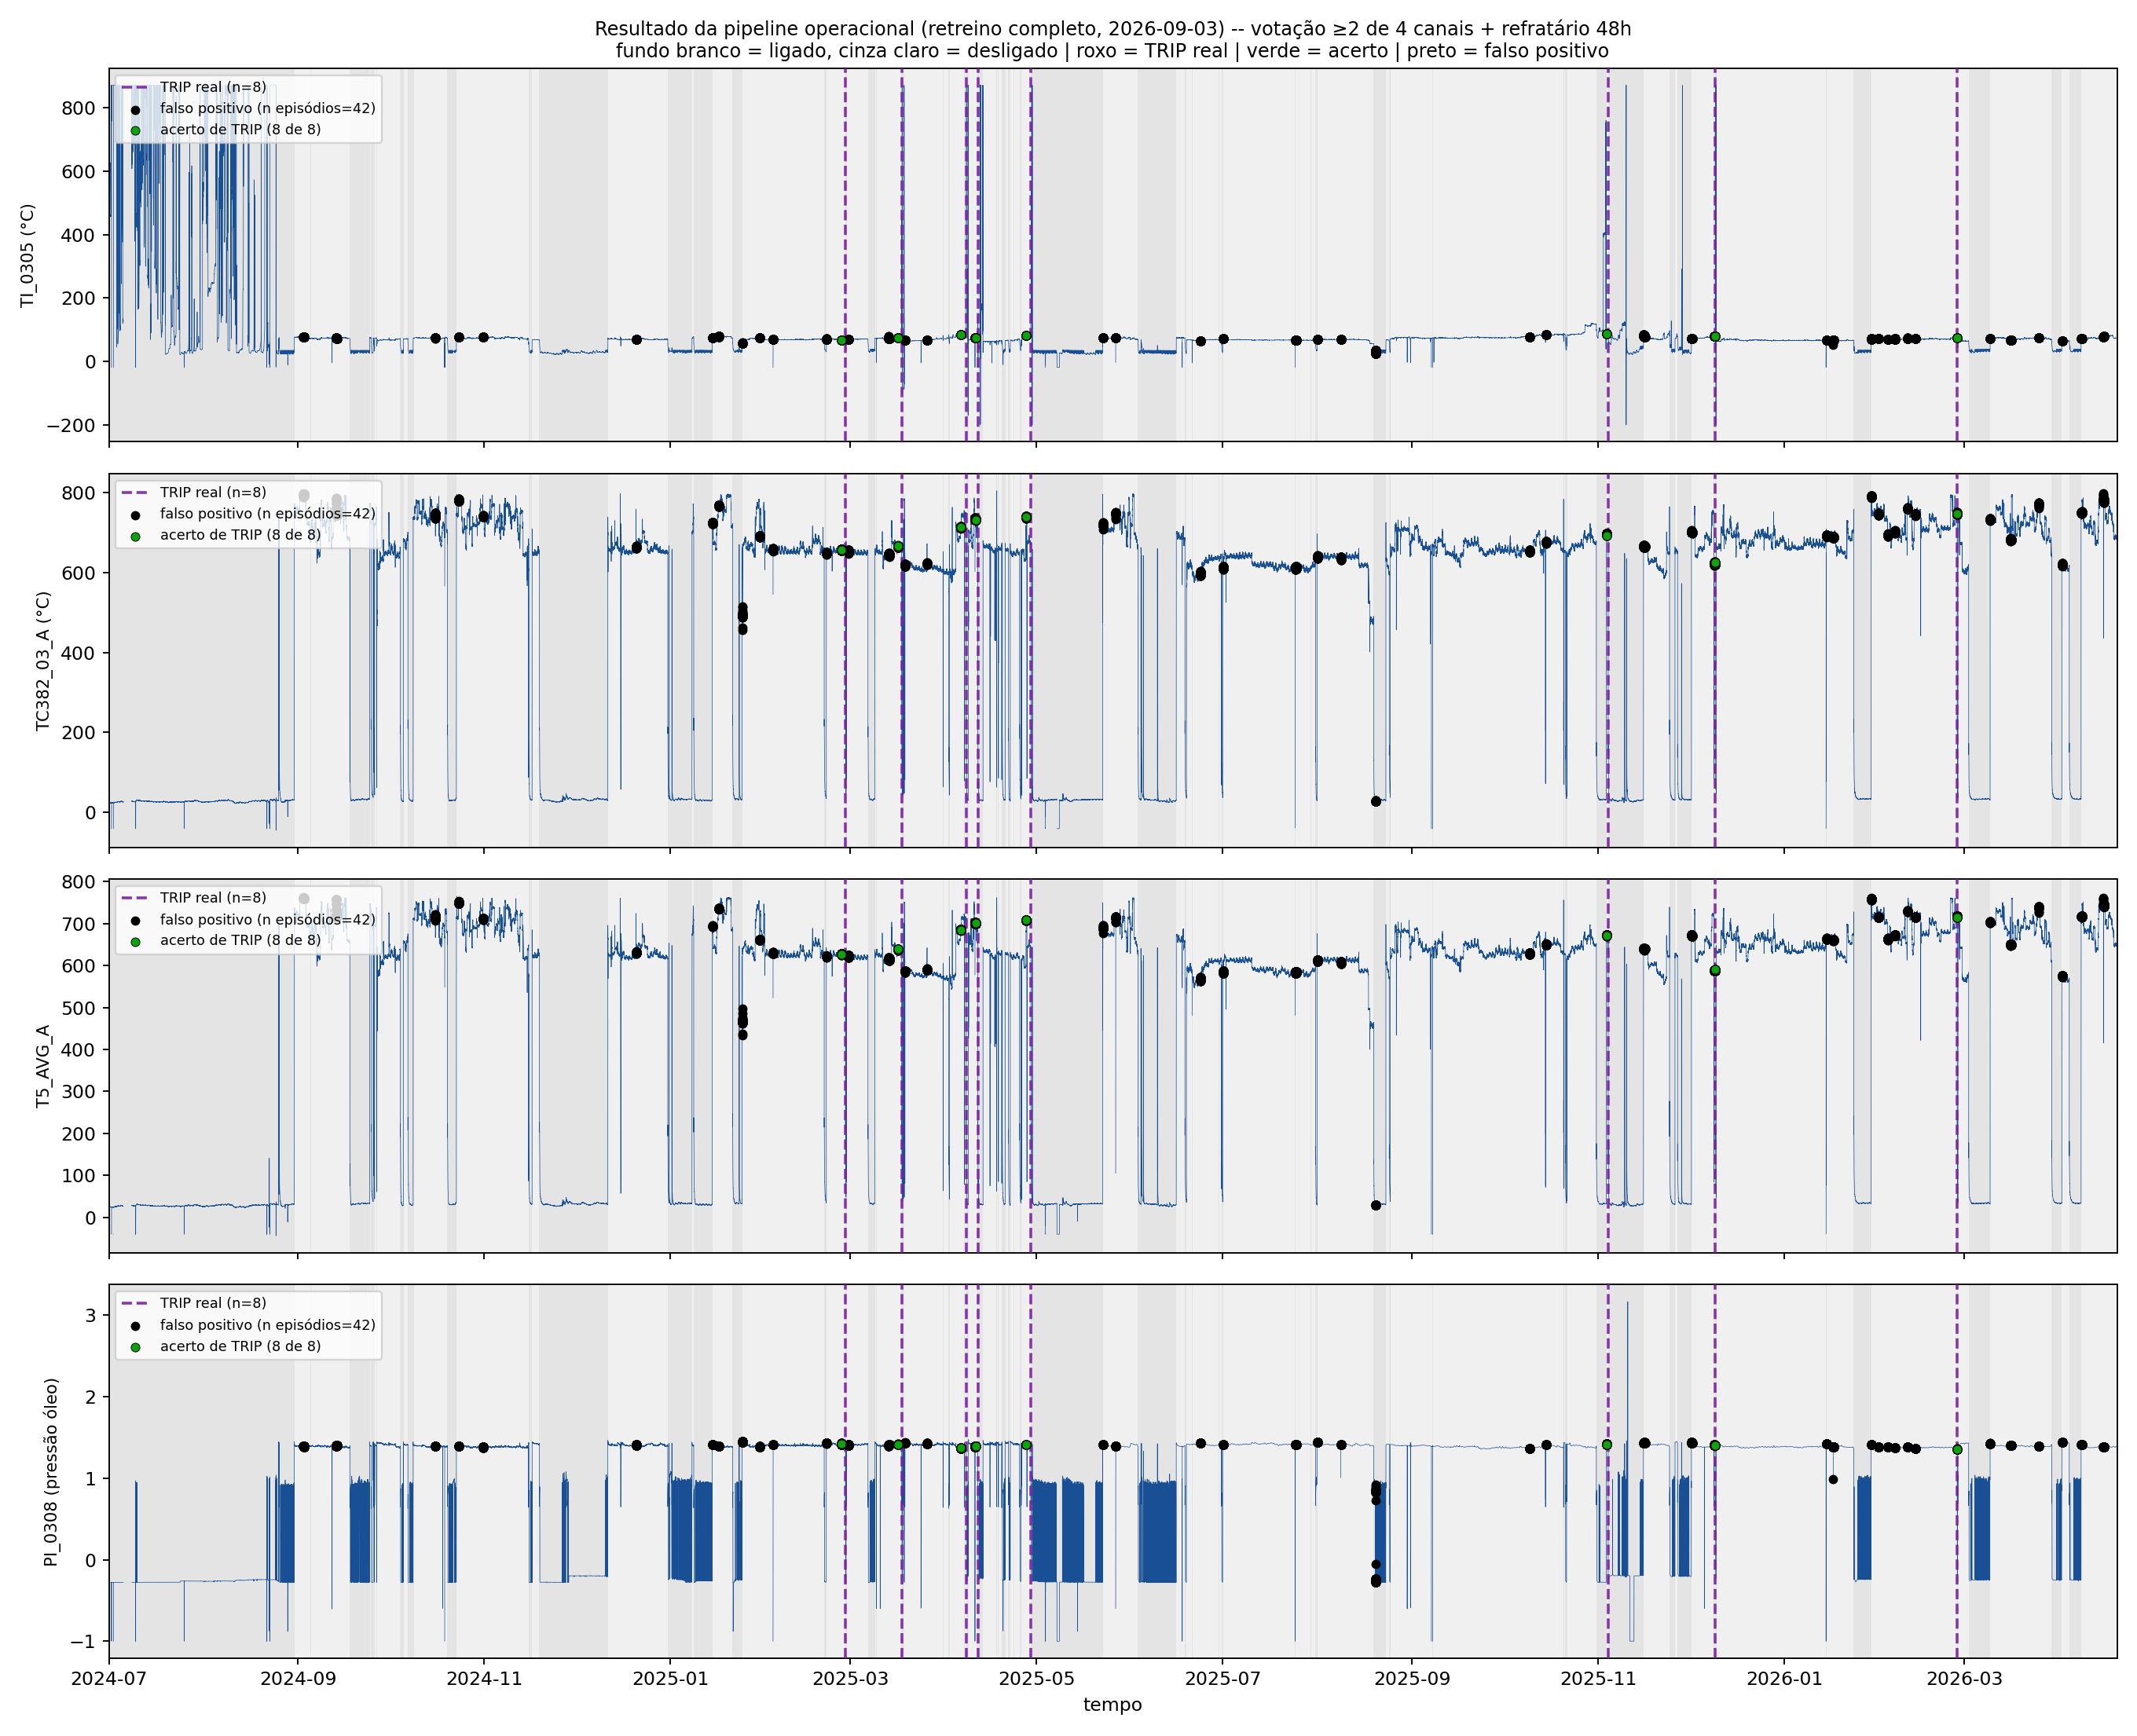
\includegraphics[width=\textwidth]{resultado_operacional_serie.png}
\caption{Série bruta (TI\_0305, TC382\_03\_A, T5\_AVG\_A, PI\_0308)
com a decisão final da pipeline (já com o filtro de duração mínima de
45min): linhas verticais roxas = TRIPs reais; pontos verdes = acerto
(8 de 8); pontos pretos = falso positivo remanescente (42 episódios,
eram 96 antes do filtro); faixas cinza = turbina desligada.}
\end{figure}

\section{Auditoria dos 42 FP remanescentes: sinal físico ou ruído?}
\label{sec:auditoria42}

A Seção~\ref{sec:estudo-fp} deixou uma pergunta em aberto: os 42
falsos positivos que sobram depois do filtro de 45min são ruído do
modelo, ou são eventos físicos reais que simplesmente não escalaram
para um TRIP catalogado? A resposta importa porque muda o que fazer a
seguir -- se for ruído, ainda há o que suprimir com segurança; se for
sinal real, suprimir mais seria apagar informação que o operador
provavelmente quer ver. Esta seção documenta a auditoria feita para
responder isso, passo a passo, com duas linhas de evidência
independentes.

\subsection{Passo 1 -- seleção dos episódios}

Os 42 episódios classificados como \texttt{falso\_positivo} pela
régua rigorosa (Seção~\ref{sec:resultado}) foram listados com seus
instantes exatos de início e fim. Ao contrário dos episódios curtos
do checkup anterior (Apêndice A do relatório de investigação, quase
pontuais), estes têm duração real: de 48 minutos a 9,65 horas --
consequência direta do filtro de 45min, que só deixa passar
concordâncias sustentadas.

\subsection{Passo 2 -- checkup de sinal físico (z-score contra baseline)}

Para cada episódio, comparou-se o comportamento dos sensores durante
a janela do episódio contra um \textbf{baseline de 2 horas
imediatamente antes} (terminando 3 minutos antes do início, para não
contaminar o baseline com o próprio início do evento). O conjunto de
sensores checados inclui todo o grupo de mancal (temperatura e os 10
canais de vibração) mais os dois sensores de óleo -- mais amplo que
os sensores do modelo que efetivamente disparou o alarme, para não
deixar passar despercebido um sinal em outro sensor correlato.

\textbf{Um cuidado metodológico que mudou o resultado}: a primeira
tentativa comparou a \emph{média} de todo o episódio contra o
baseline. Como esses episódios podem durar horas, um pico breve real
no meio de uma janela longa fica diluído pela média -- e o resultado
saiu artificialmente baixo (21,4\% ``confirmado''). Corrigido para
usar o \textbf{pico máximo pontual} dentro do episódio (o critério
correto, coerente com como o próprio modelo de anomalia reage a
picos, não a médias), o resultado mudou para:

\begin{table}[H]
\centering
\begin{tabular}{lc}
\toprule
\textbf{Classificação} & \textbf{\% dos 42} \\
\midrule
Confirmado real (forte: $|z|\geq10$ e $\geq$2 sensores) & 26,2\% (11) \\
Confirmado real (moderado: $|z|\geq3$ e $\geq$2 sensores) & 35,7\% (15) \\
Borderline (só 1 sensor com $|z|\geq3$) & 28,6\% (12) \\
Fraco / sem explicação física & 9,5\% (4) \\
\bottomrule
\end{tabular}
\caption{Checkup individual dos 42 FP -- pico de z-score dentro do
episódio contra baseline de 2h. \textbf{61,9\% confirmados reais}
(forte+moderado), consistente com os 79\% já encontrados nos 24
episódios isolados do relatório de investigação.}
\end{table}

Apenas 4 episódios não mostram nenhuma explicação física em nenhum
sensor checado -- únicos candidatos honestos a ruído puro:
\texttt{2025-01-14\_17h57}, \texttt{2025-01-24\_12h42},
\texttt{2025-02-21\_03h27} e \texttt{2026-03-09\_12h07}.

\subsection{Passo 3 -- segunda evidência: corroboração por outro alarme de processo}

Sinal físico no próprio sensor é uma evidência; uma segunda e
independente é verificar se \textbf{outro alarme do processo}, já
catalogado pela planta, ocorreu perto do mesmo instante -- ou seja,
se o próprio sistema de alarmes da Cabiúnas também percebeu algo ali,
por um caminho diferente do nosso modelo.

Usou-se o catálogo completo (47 tags, 3.757 ocorrências ativas no
período), \textbf{excluindo os 5 tags já usados no canal de alarme
da própria pipeline} (para não contar a mesma evidência duas vezes) e
uma janela de $\pm$2h.

\textbf{Controle negativo obrigatório}: uma taxa alta de ``explicado
por outro alarme'' só é evidência real se for muito maior do que a
taxa que apareceria em instantes aleatórios -- do contrário, é só
reflexo de um catálogo denso (mesmo cuidado já aplicado nesta
investigação para o enriquecimento por catálogo, Seção~2 do
relatório de investigação). Comparou-se a taxa nos 42 FP contra
5.000 instantes aleatórios do período monitorado:

\begin{table}[H]
\centering
\begin{tabular}{lc}
\toprule
\textbf{Grupo} & \textbf{Taxa (outro alarme em $\pm$2h)} \\
\midrule
42 FP (pós-filtro 45min) & \textbf{23,8\% (10 de 42)} \\
Baseline aleatório (5.000 amostras) & 3,4\% \\
\midrule
\textbf{Enriquecimento} & \textbf{6,9$\times$} \\
\bottomrule
\end{tabular}
\caption{Corroboração por outro alarme de processo, com controle
negativo. Um enriquecimento de 6,9$\times$ é forte -- bem acima de
1,0$\times$ (que indicaria catálogo denso demais para discriminar) --
não é artefato.}
\end{table}

\begin{figure}[H]
\centering
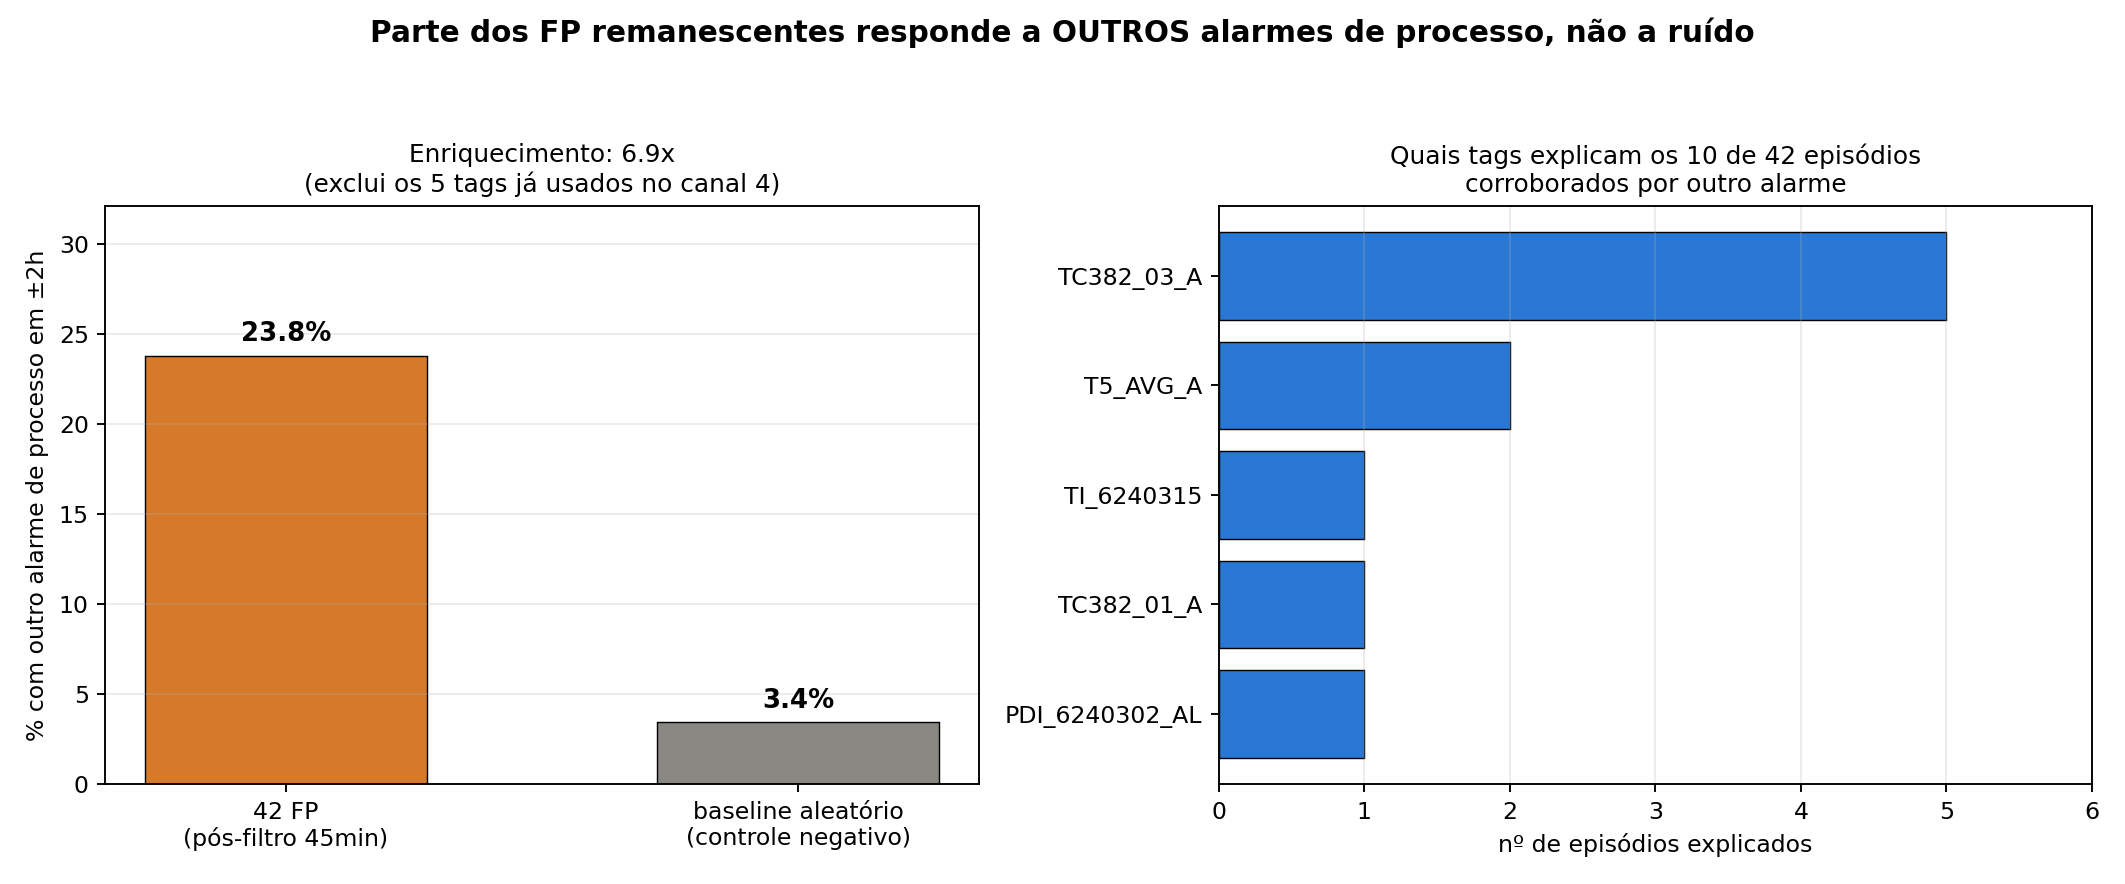
\includegraphics[width=\textwidth]{alarmes_proximos_42fp.png}
\caption{Esquerda: taxa de corroboração por outro alarme nos 42 FP
vs. baseline aleatório (controle negativo). Direita: quais tags do
catálogo explicam os 10 episódios corroborados -- concentradas em
alarmes do próprio sensor de temperatura de mancal
(\texttt{TC382\_03\_A}, \texttt{T5\_AVG\_A}).}
\end{figure}

\subsection{Passo 4 -- visualização na série completa}

A Figura~\ref{fig:auditoria42} mostra as duas evidências sobrepostas
na série bruta inteira: os 10 FP corroborados por outro alarme
aparecem em azul, com uma linha pontilhada fina marcando o instante
exato desse outro alarme (não é TRIP -- é um alarme de processo
diferente, catalogado pela planta); os 32 FP sem essa corroboração
específica continuam em preto (a maioria deles ainda tem sinal físico
próprio confirmado pelo Passo 2, só não bateu com outro alarme do
catálogo em $\pm$2h).

\begin{figure}[H]
\centering
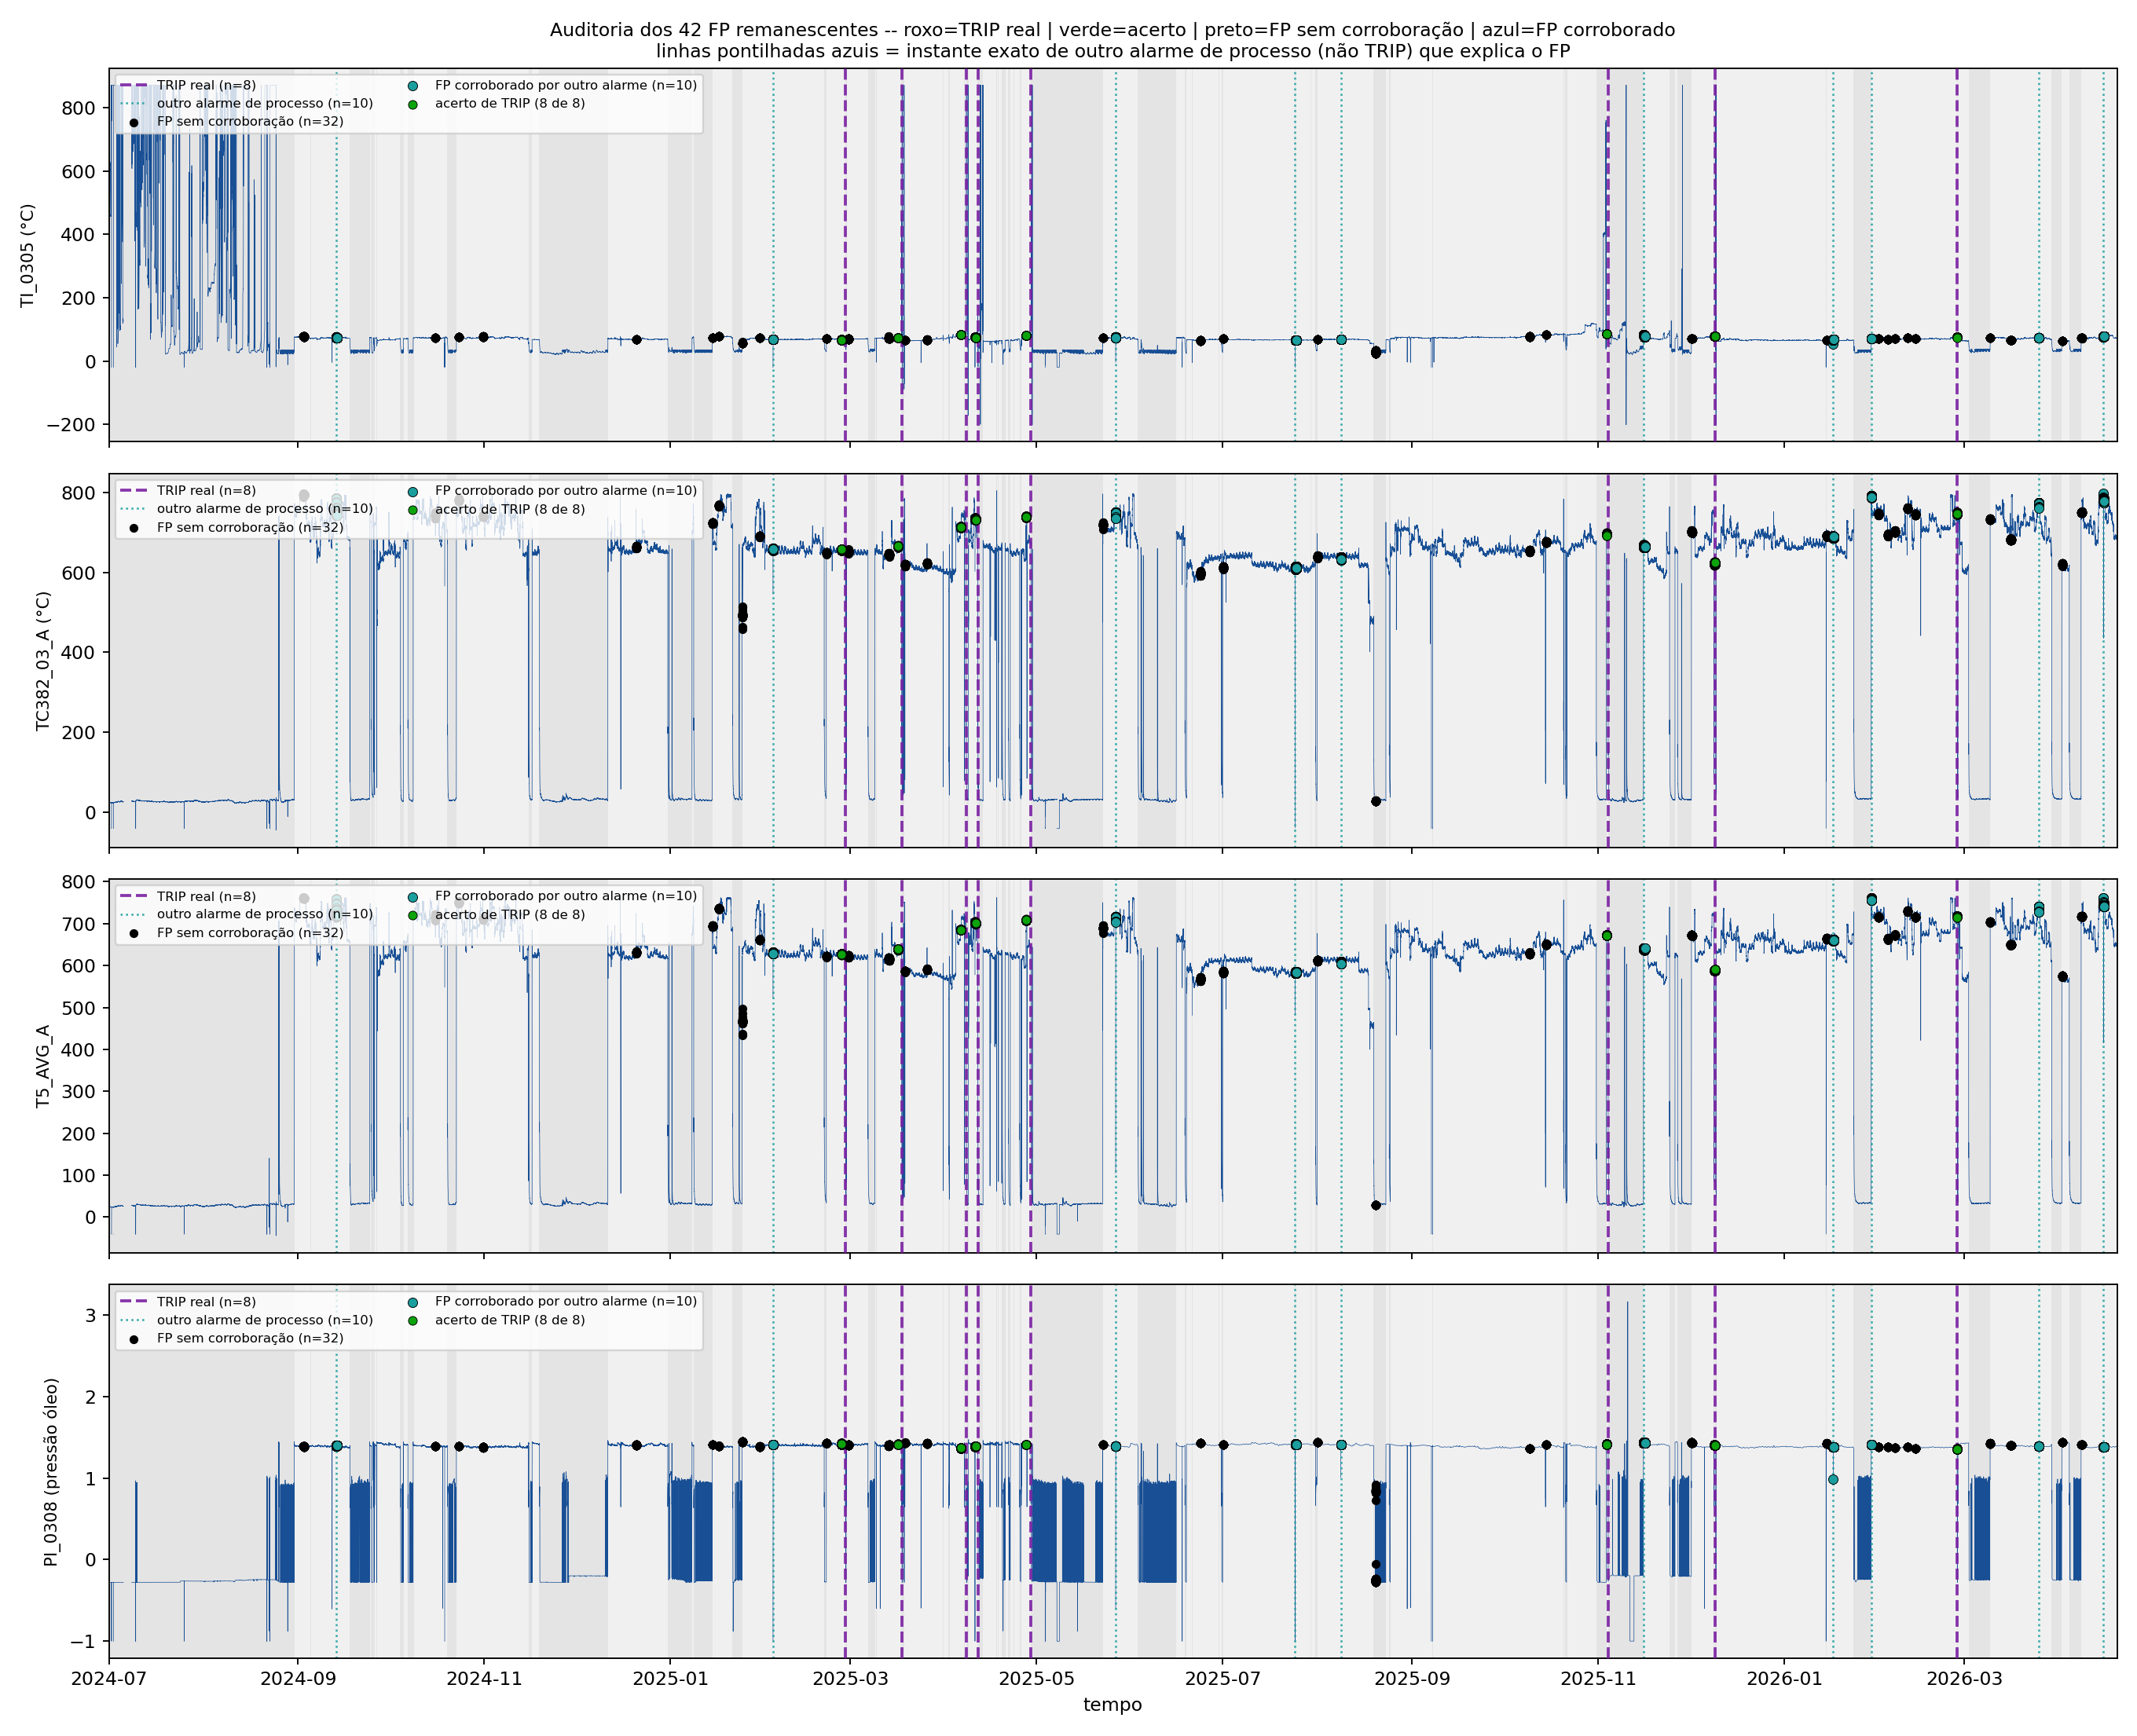
\includegraphics[width=\textwidth]{serie_auditoria_42fp.png}
\caption{Série bruta completa com a auditoria dos 42 FP: roxo = TRIP
real; verde = acerto; preto = FP sem corroboração por outro alarme;
azul = FP corroborado; linhas pontilhadas azuis finas = instante
exato do outro alarme de processo que explica cada FP corroborado.}
\label{fig:auditoria42}
\end{figure}

\subsection{Conclusão da auditoria}

Combinando as duas linhas de evidência independentes -- 90,5\% dos
42 FP com sinal físico próprio (confirmado ou borderline) e 23,8\%
também corroborados por outro alarme de processo já catalogado --
fica difícil defender que os FP remanescentes sejam ruído do modelo.
São, na maioria, \textbf{eventos físicos reais que a própria planta
às vezes também registra}, mas que não escalaram para um TRIP
catalogado desta vez. \textbf{Recomendação: não suprimir mais} --
2,88 FP/mês é um teto honesto, não apenas técnico. Os 4 episódios sem
nenhuma explicação (Passo 2) são os únicos candidatos legítimos a uma
investigação futura mais específica.

\section{Reprodução operacional}

Todo o resultado deste documento é reproduzível a partir do
repositório, sem passos manuais além de submeter os jobs de
treinamento:

\begin{itemize}
  \item \textbf{Configs de treino}:
    \texttt{configs/calibracao\_v4\_eq/test\_grupo\_exp33\_mancal\_temperatura\_isolada.json},
    \texttt{test\_grupo\_exp34\_mancal\_vibracao\_isolada.json},
    \texttt{test\_grupo\_exp38\_oleo\_pressao\_isolada.json}.
  \item \textbf{Treino}: \texttt{PYTHONPATH=. python src/main.py --config <config>.json}
    para cada um dos 3 canais (envia para a fila remota do ClearML).
  \item \textbf{Decisão final}: \texttt{PYTHONPATH=. python
    scripts/pipeline\_unificada\_final.py} -- baixa os 3
    \texttt{point\_anomalies\_all.csv} já treinados, monta o canal de
    alarme, aplica votação e refratário, e escreve o resultado final
    em \texttt{runs\_pipeline\_unificada\_final/}.
  \item \textbf{Retreino completo confirmado em 03/09/2026}: os três
    modelos foram retreinados do zero (novas tasks no ClearML) e o
    resultado final (antes do filtro de duração mínima) foi idêntico
    -- 8/8 TRIPs, 6,59 FP/mês, mesmos instantes de detecção --
    confirmando que a pipeline é reprodutível ponta a ponta.
  \item \textbf{Filtro de duração mínima adicionado em 04/09/2026}
    (Seção~\ref{sec:estudo-fp}): 45 minutos aplicados à votação
    combinada, via \texttt{apply\_min\_duration\_filter} (já existente
    em \texttt{src/cnn1d\_ae/scoring.py}, antes usado só por canal) --
    reduz FP/mês para 2,88 mantendo 8/8.
\end{itemize}

\end{document}
